\newcommand{\institut}{Institut f\"ur Telekommunikationssysteme}
\newcommand{\fachgebiet}{Nachrichten\"ubertragung}
\newcommand{\veranstaltung}{Praktikum Nachrichten\"ubertragung}
\newcommand{\pdfautor}{Dirk Babendererde (321 836), Thomas Kapa (325 219)}
\newcommand{\autor}{Dirk Babendererde (321 836)\\ Thomas Kapa (325 219)}
\newcommand{\gruppe}{Gruppe:}
\newcommand{\betreuer}{Betreuer: Lieven Lange}


\newcommand{\pdftitle}{Nachrichtenuebertragung\ Praktikum\ 03}
\newcommand{\prototitle}{Praktikum 03 \\ Statistische Nachrichtentheorie}

\input{../../packages/tu_header_9}
%\begin{document}


%     \lstinputlisting{./praktikum6.sce}

%---------------------------------------------------------------------
%---------------------------------------------------------------------
%---------------------------------------------------------------------


\section{Vorbereitungsaufgaben}
\begin{quote}
    \hspace{-2em}
    \subsection{Herleitung der Spektren}
    \begin{quote}
        
        \subsubsection{Shape-Top-Abtastung}
        \begin{quote}
            
            
            \begin{equation*}
                \begin{split}
                    f_m (t)   &= f(t) \cdot \sqcap_{\alpha T} (t) \ast \delta_T (t) \\
                    F_m (j\omega) &= \frac{1}{2\pi} F (j\omega) \ast \left [ \alpha T \cdot si \left( \frac{\omega
                    \alpha T}{2} \right) \cdot \omega_T \cdot \delta_{\omega T} (\omega) \right] \\
                    &= \alpha \cdot F (j \omega) \ast \left ( si \left( \frac{\omega \alpha T}{2} \right)
                    \sum_{k=-\infty}^{\infty} \delta (\omega - k\omega_T) \right)\\
                    &= \alpha \cdot F (j \omega) \ast \sum_{k=-\infty}^{\infty} (si(k \pi \alpha) \cdot \delta (\omega -
                    k\omega_T))\\
                    &= \alpha \cdot \sum_{k=-\infty}^{\infty} \left [ si(k \pi \alpha) \cdot F (j(\omega - k\omega_T))
                    \right]\\
                    \label{eq:shape}
                \end{split}
            \end{equation*}
            
            
        \end{quote}
        
        \subsubsection{Flat-Top-Abtastung}
        \begin{quote}
            
            
            \begin{equation*}
                \begin{split}
                    f_m (t) &= [f (t) \cdot \delta_T (t)] \ast \sqcap_{\alpha T} (t)\\
                    F_m (j\omega) &= \left ( \frac{1}{2 \pi} F (j\omega) \ast \omega_T \cdot \delta_T (\omega) \right) \cdot
                    \alpha T \cdot si (\frac{\alpha \omega T}{2})\\
                    &= \alpha \cdot si \left( \frac{\omega \alpha T}{2} \right) \cdot \sum_{k=-\infty}^{\infty} F(j(\omega -
                    k\omega_T))\\
                    \label{eq:flat}
                \end{split}
            \end{equation*}
            
            
        \end{quote}
        
        
    \end{quote}
    
    
    \subsection{Skizzieren}
    \begin{quote}
        Zur übung das Spektrum folgenden Signals
        
        \begin{equation*}
        	\begin{split}
                f(t) = A \p cos(\frac{\omega_T}{5} t)
        	\end{split}
        \end{equation*}
        
        mit $\alpha = 0,5$ und $\omega_T =$ \SI{20}{\pi\ \kilo\hertz} Skizzieren.
        
        
        \begin{figure}[H]
        \centering\fbox{
            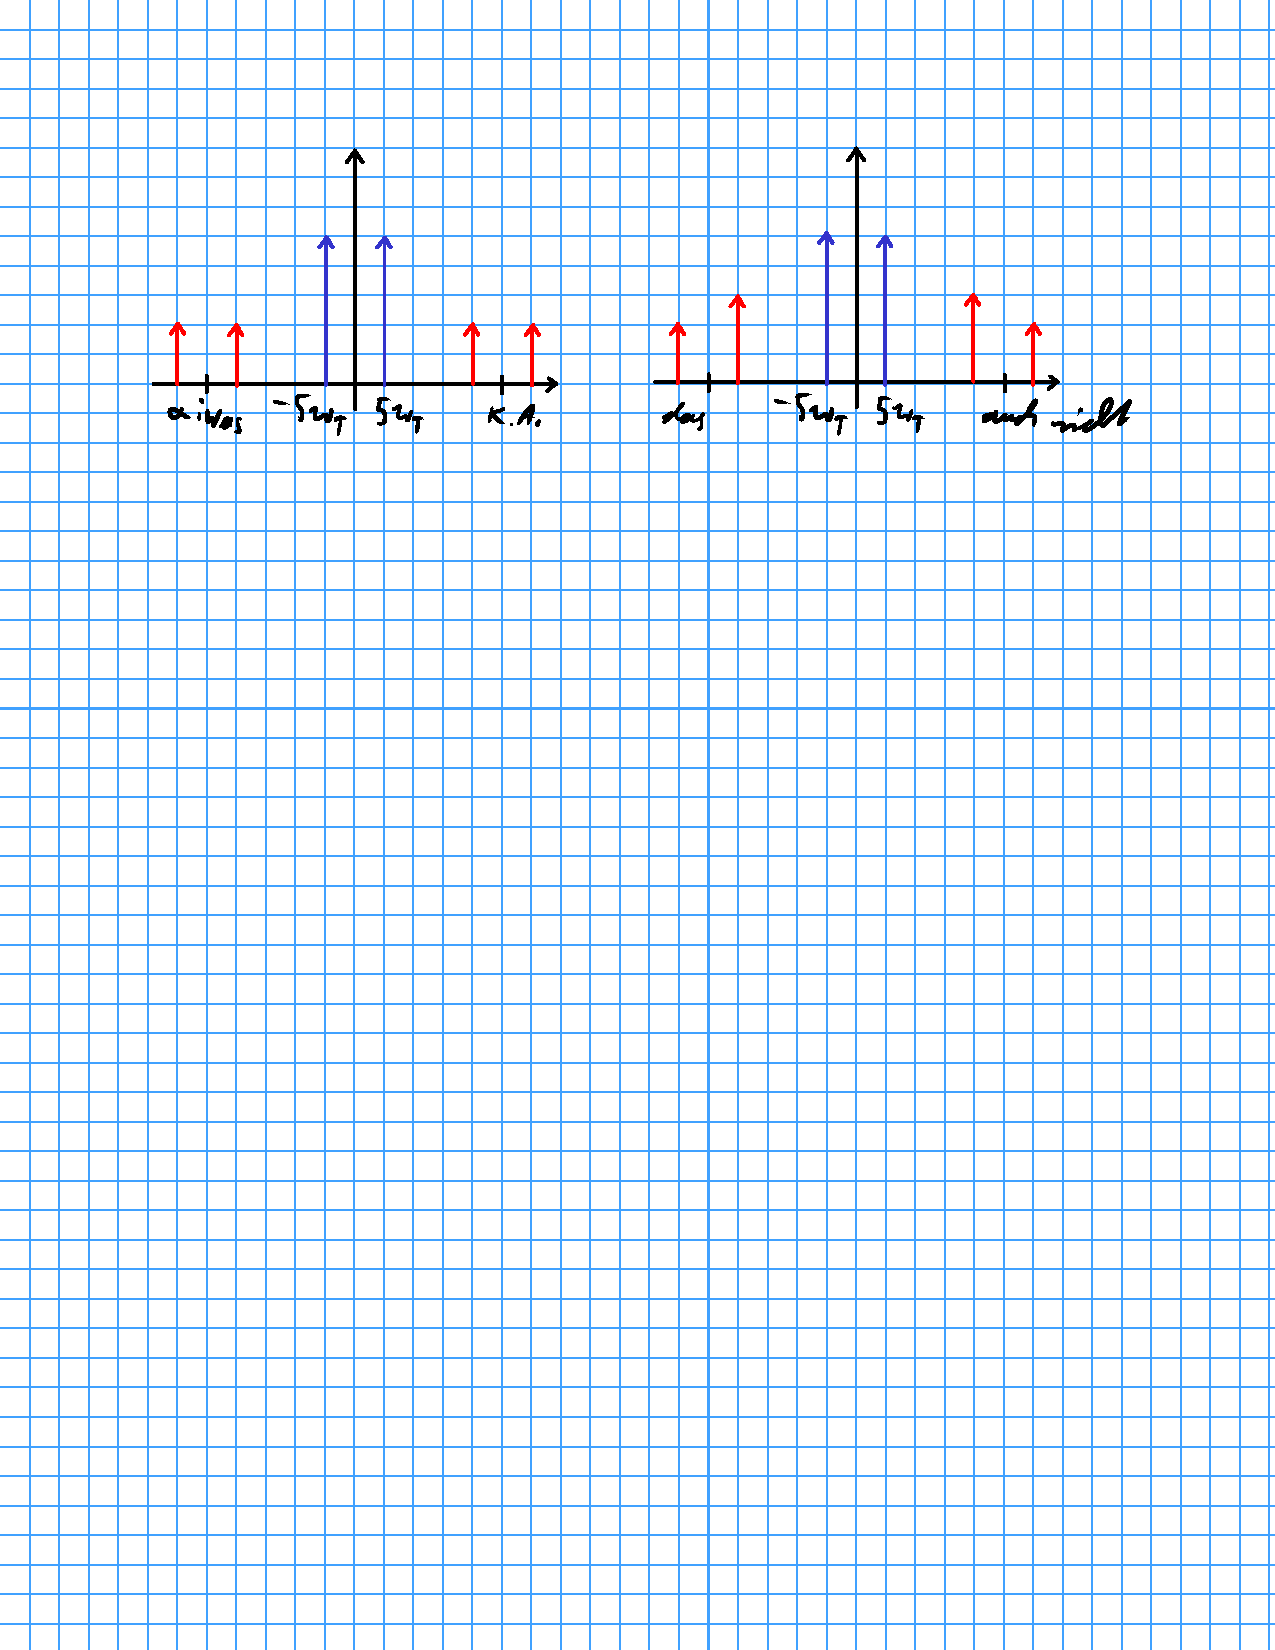
\includegraphics[scale=0.7, trim = 1cm 18cm 1cm 2cm, clip]{Bilder/skizze}}
                \caption{sampling Skizze}
                \label{fig:skizze}
        \end{figure}
        
        
    \end{quote}
    
    
    \subsection{MatLab-Simulation}
    \begin{quote}
        Um unsere Durchführungsergebnisse mit idealen Werten vergleichen zu können haben wir die Praktikumsaufgaben in
        Matlab simuliert.
        
         \TODO{Hier müssen noch die Bilder mit sinnvoller Darstellung eingefügt werden????}
         
    \end{quote}
    
    
\end{quote}

%--------------------------------------------------------------------
%--------------------------------------------------------------------


\section{Durchführung}
\begin{quote}
    
    
    \subsection{Labordurchführung}
    \begin{quote}
     Für die Signalausblendung (Shape-Top-Sampling) und die Signalverbreiterung (Flat-Top-Sampling) wird das Dual
     Analog Switch- Modul verwendet.
     Bei beiden Samplingvarianten wird auf den Eingang "`Control 1"' ein unipolares Rechtecksignal mit einer Spannung von 0
     bis 5 Volt, variabler Frequenz (10 und 20 Hz) und variablem Tastverhältnis (0,2 , 0,5 und 0,7) gelegt. Dieses wird
     vom Signalgenerator geliefert.
     Es sollen drei abzutastende Signale untersucht werden. Zum einen ein bipolares, mittelwertfreies Rechtecksignal mit
     einer Spitze-Spitze-Spannung von 4 Volt und einer Frequenz von 2 kHz, welches vom Master Signals Modul geliefert
     wird. Dafür wird der Ausgang 2 kHz DIGITAL verwendet. Dieser liefert allerdings ein Rechtecksignal mit der Spannung
     von 0 bis 5 Volt. Damit man das bipolare Signal erhält, wird das ADDER Modul verwendet. Das Rechtecksignal wird auf
     den Eingang B gegeben, wo das Signal mittels der Verstärkung von 4/5 auf 0 bis 4 Volt eingestellt wird. Da das
     Signal noch unipolar ist muss zuletzt ein Offset von -2 Volt mit Hilfe des Variable DC Moduls addiert
     werden.\\
     \noindent\hspace*{4mm}
     Als zweites Signal soll das eben erstellte bipolare Rechtecksignal vor der Abtastung tiefpassgefiltert werden. Dazu
     wird das RC LPF Modul, also ein Tiefpass bestehend aus einem Kondensator und einer Spule, verwendet.
     Zum anderen soll ein 2 kHz Sinussignal abgetastet werden, welches ebenfalls dem Master Signals Modul entnommen
     werden kann.\\
     \noindent\hspace*{4mm}
     Bei der Signalausblendung wird das abzutastende Signal auf den Eingang IN1 gegeben und der Ausgang am Out
     abgegriffen. Damit wird ein Schalter geöffnet und geschlossen, was dazu führt, dass die Kontur des Signals im
     Abtastpuls mit übertragen wird (daher Shape-Top).\\
     Bei der Signalverbreiterung wird das Quellensignal noch zusätzlich vorher durch ein S\&H-Glied, also ein Abtast-
     und Halteglied (S\&H IN, S\&H OUT) und von da aus in IN1 geführt. Dieses sorgt dafür, dass bei einem Abtastimpuls
     nur ein Wert durchgängig übertragen wird (daher Flat-Top).\\
     \noindent\hspace*{4mm}
     Zuletzt wird das Signal zur Rekonstruktion noch durch einen Tiefpassfilter mit variabler Grenzfrequenz geführt
     (TUNEABLE LPF IN/OUT).\\
     \noindent\hspace*{4mm}
     Für die Messungen wird das Abtastsignal sowohl in der Frequenz, als auch im Tastgrad, wie oben gegeben für
     Signalverbreiterung und Signalausblendung variiert.
     Dabei kann man einige der Kombinationen auslassen. Da sich z.B. die Veränderungen von $\alpha$ bei 10 und 20 kHz
     ähnlich auswirken, wird im Versuch nur der Tastgrad für 20 kHz variiert.\\
     \noindent\hspace*{4mm}
     Im zweiten Teil soll ein Sprachsignal mit Signalausblendung oder Signalverbreiterung abgetastet werden. Dazu wird
     ein Mikrofon des SPEECH Modul genutzt und beim BUFFER Modul ein Kopfhörer angeschlossen.
    \end{quote}
    
\end{quote}


\section{Auswertung \& Theorie}
\begin{quote}
    
    Im Labor haben wir dann folgende Messungen durchgefüht.
    
    
    \subsection{Flat-Top Sampling}
    \begin{quote}
        
        \subsection{Änderung der Trägerfrequenz}
        \begin{quote}
            
            Der Theorie nach sollte das Signal, das mit einer höheren Frequenz abgestastet wird, auf Grund der Mehrzahl
            an Stützstellen auch besser rekonstruiert werden.
            Das reine Rechtecksignal sollte ein starkes Überschwingen zeigen, da es unendlich viele Frequenzanteile
            enthält und das Abtasttheorem für die großen Frequenzen nicht eingehlten werden kann.
            Das tiefpassgefilterte Rechtecksignal sollte aufgrund der entnommenen hohen Frequenzen weniger Überschwingen
            nach der rekonstruktion enthalten.
            Der nahezu reine Sinus sollte ziemlich gut rekonstruiert werden können, da er theoretisch nur einen
            Frequenzanteil enthält. Alle Wiederholungen des Spektrums können somit sehr einfach weggefiltert werden.
            
            \TODO{Soll überhaupt noch ein Sinus eingefügt werden????}
            \TODO{Thommy: was? wo eingefügt?}
            
            \begin{center}
            \begin{tabular}{ll}
            
            \hspace{-5cm}
                \begin{minipage}{0.6\textwidth}
                    \begin{figure}[H]
                        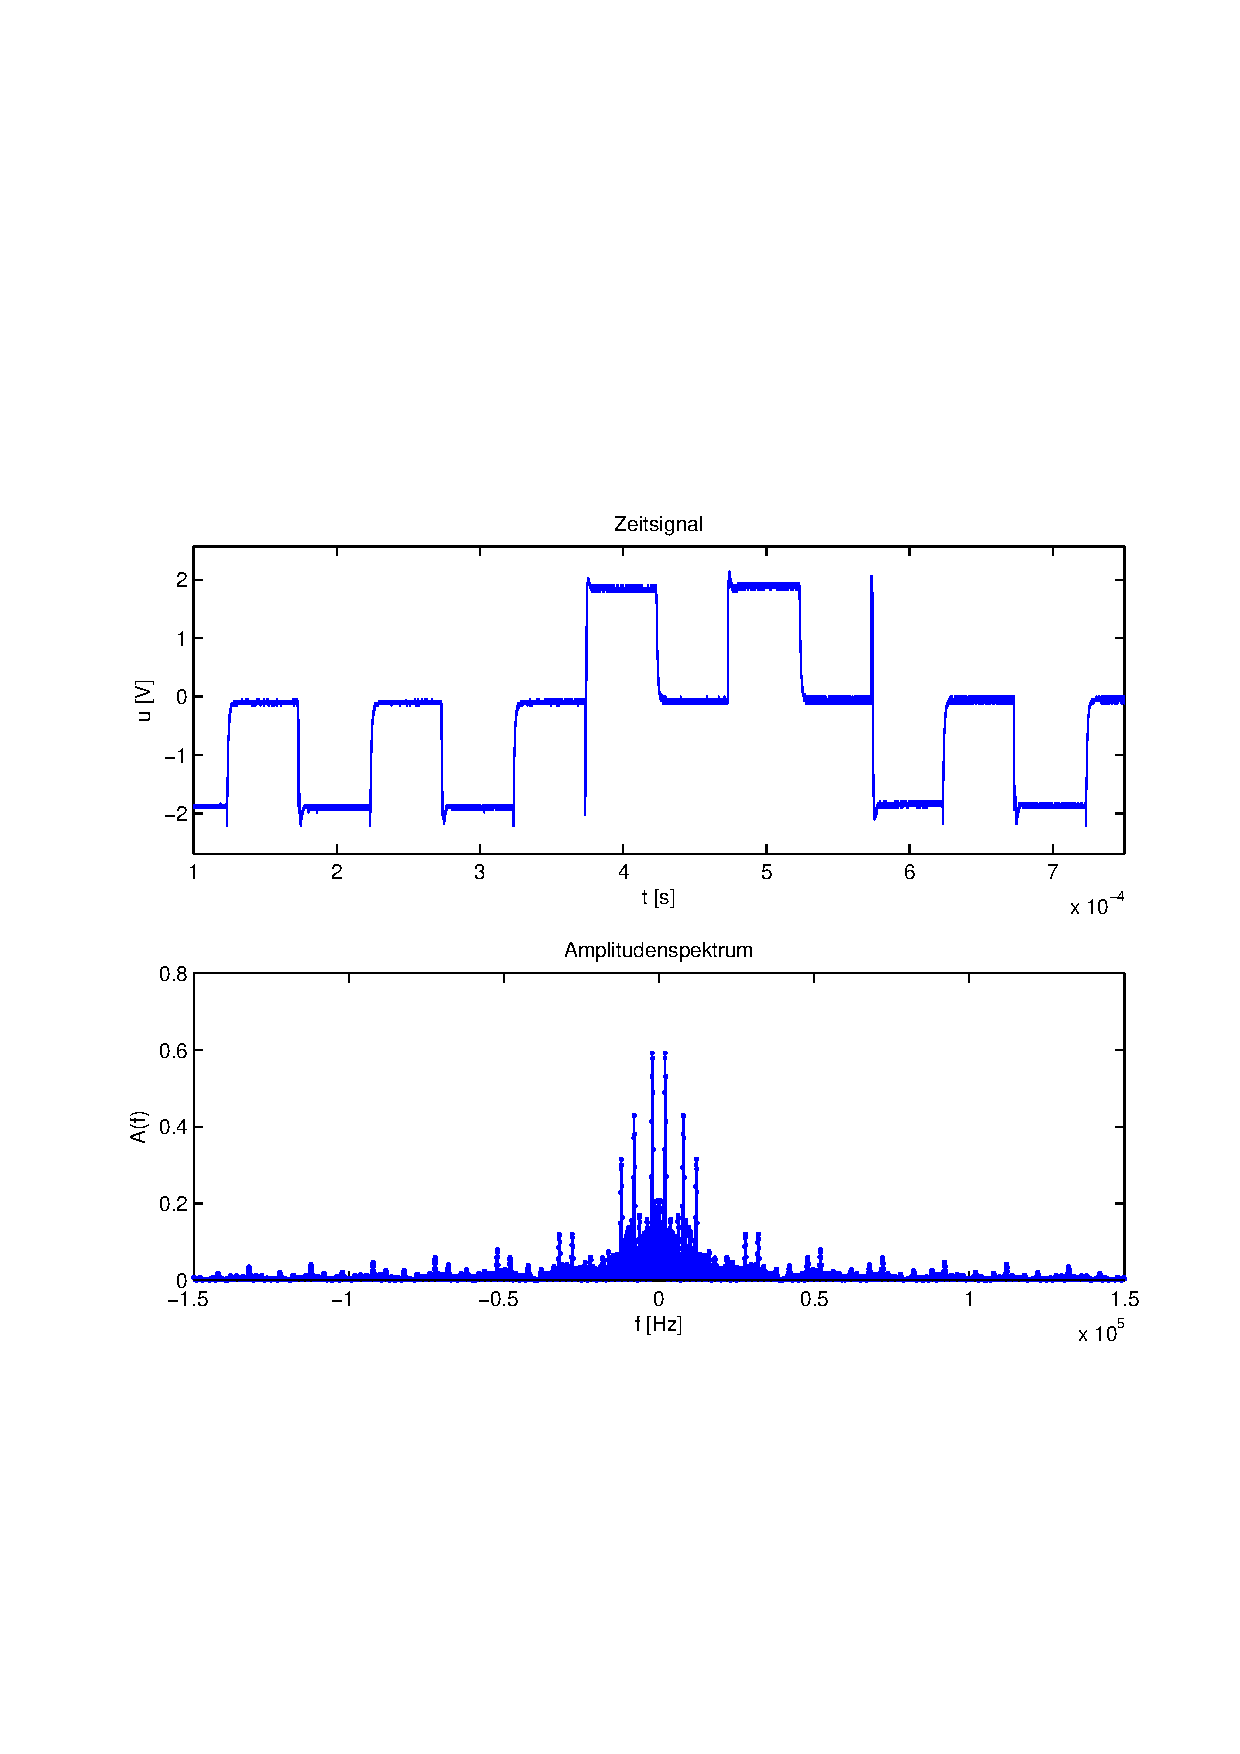
\includegraphics[scale=0.7, trim = 35mm 100mm 35mm 95mm, clip]{Bilder/flatrec10_05abget_zeit}
                          \caption{Rechteck 10 kHz alpha 0,5 moduliertes Signal}
		                  \label{fig:flatrec10_05zeit}
                    \end{figure}
                \end{minipage}
                
                \begin{minipage}{0.6\textwidth}
                    \begin{figure}[H]
                        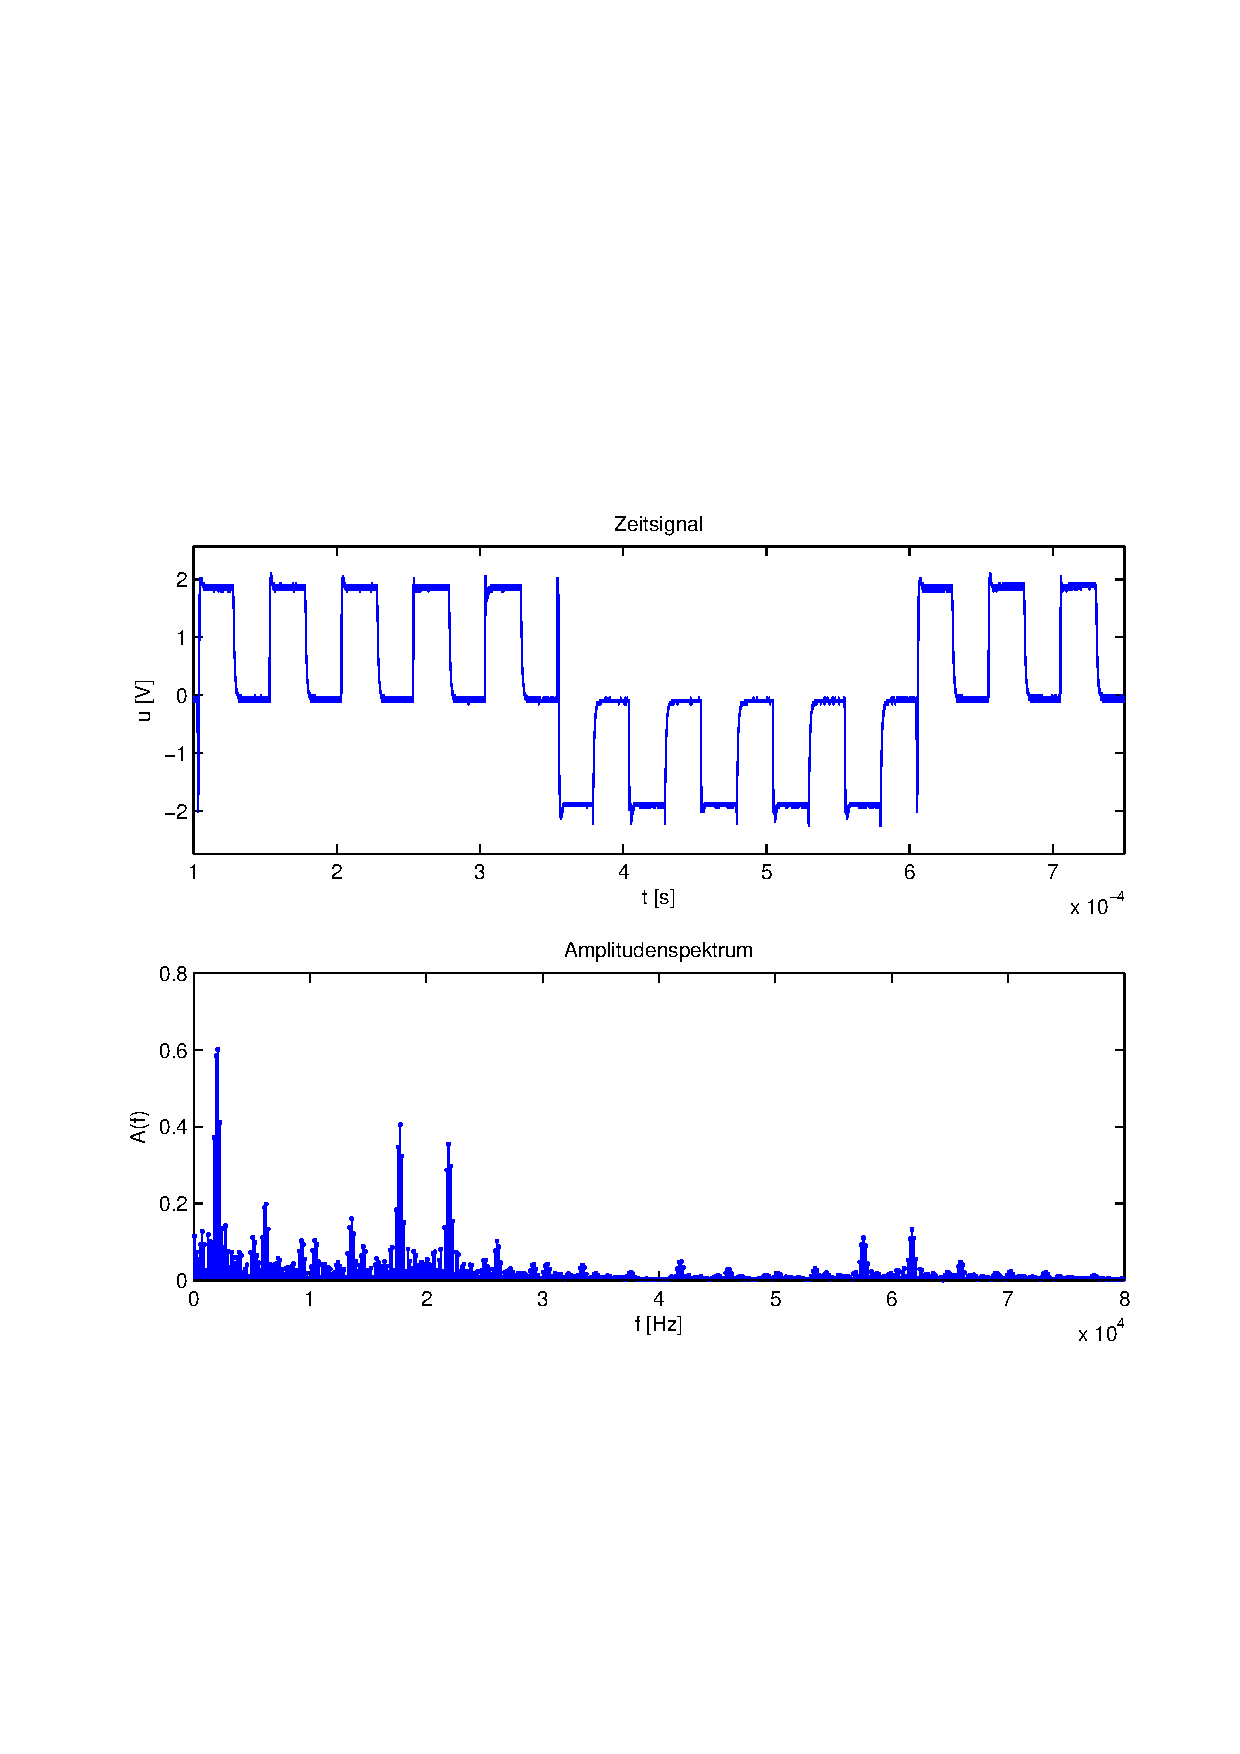
\includegraphics[scale=0.7, trim = 35mm 100mm 35mm 95mm, clip]{Bilder/flatrec20_05abget_zeit}
                       \caption{Rechteck 20 kHz alpha 0,5 moduliertes Signal}
		              \label{fig:flatrec20_05zeit}
                    \end{figure}
                \end{minipage}
            
            \end{tabular}
            \end{center}
            
            \begin{center}
            \begin{tabular}{ll}
            
            \hspace{-5cm}
                \begin{minipage}{0.6\textwidth}
                    \begin{figure}[H]
                        
\includegraphics[scale=0.7, trim = 35mm 100mm 35mm 95mm, clip]{Bilder/flatrec10_05}
                          \caption{Rechteck 10 kHz alpha 0,5 Rekonstruktion}
		                  \label{fig:flatrec10_05}
                    \end{figure}
                \end{minipage}
                
                \begin{minipage}{0.6\textwidth}
                    \begin{figure}[H]
                        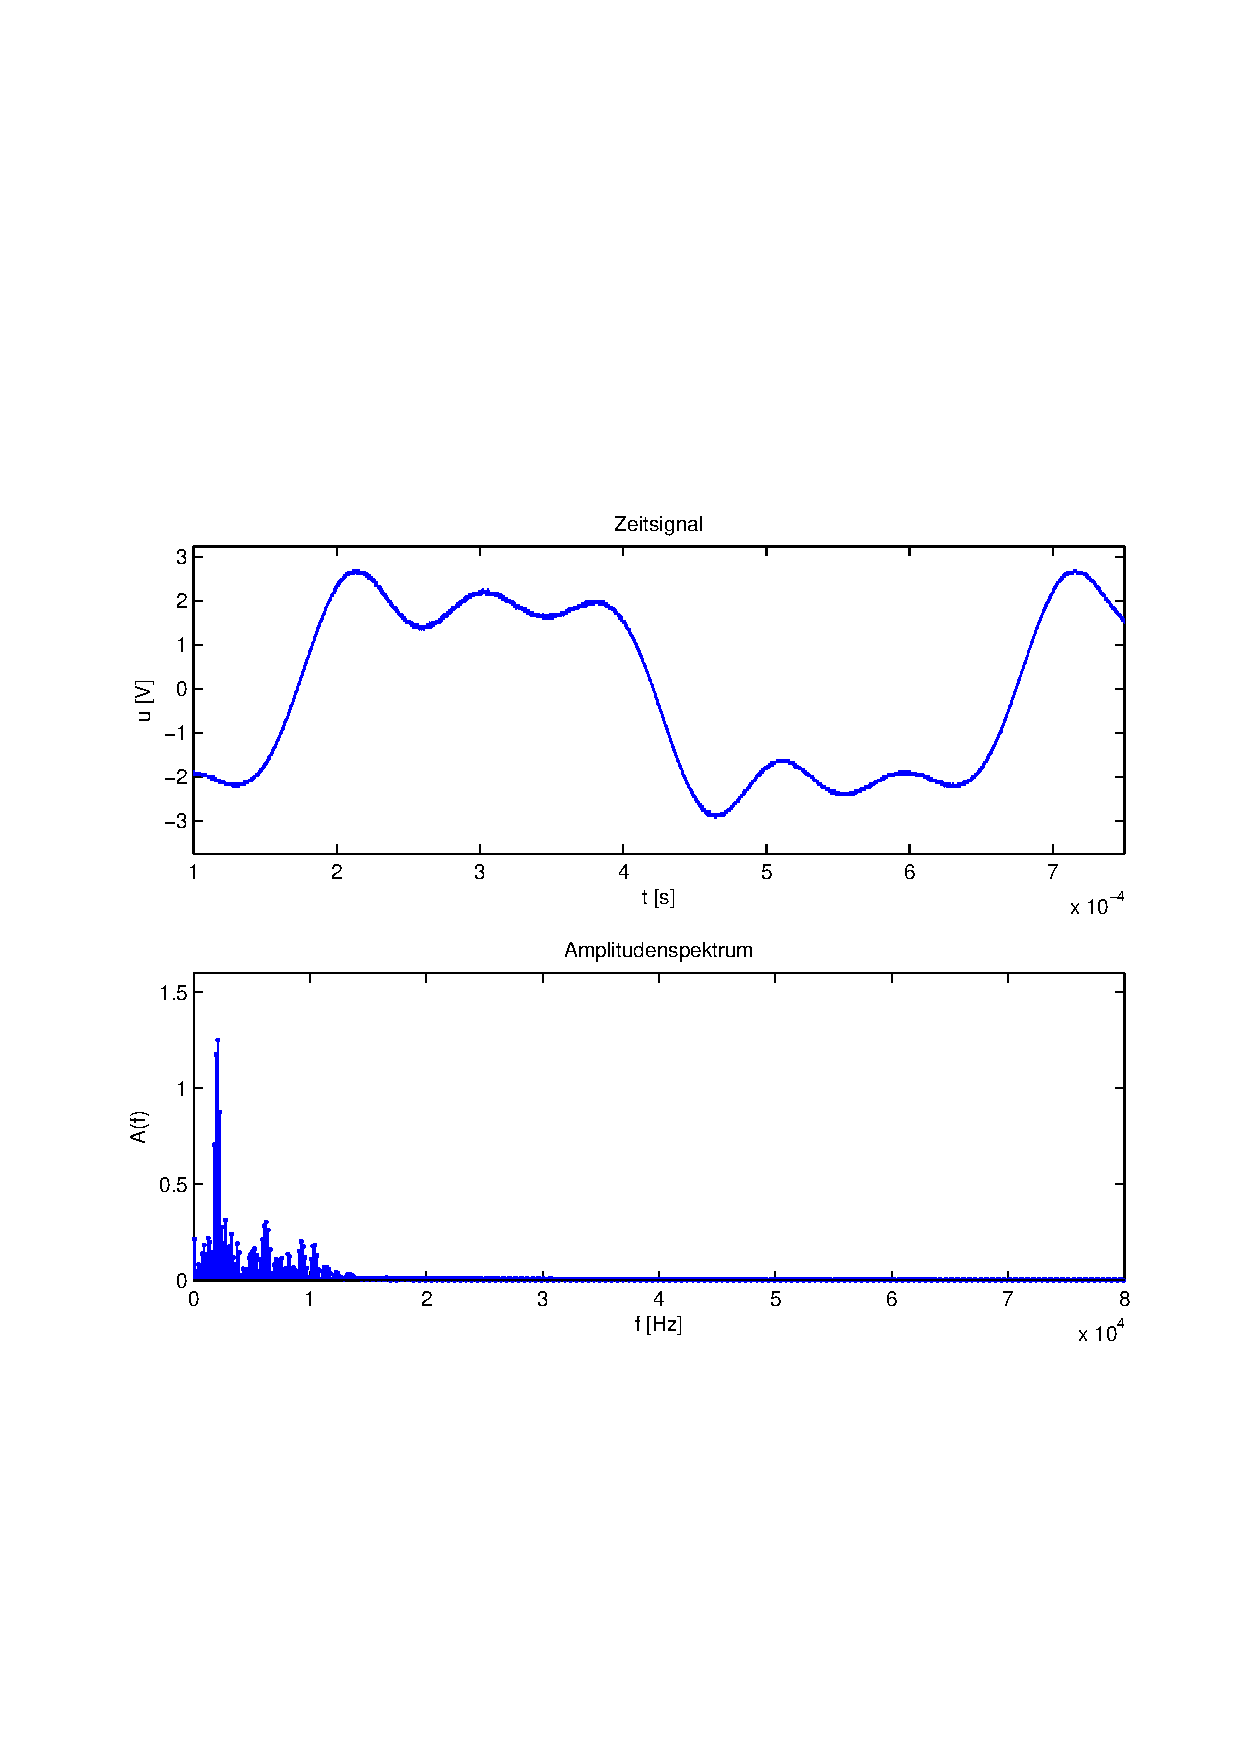
\includegraphics[scale=0.7, trim = 35mm 100mm 35mm 95mm, clip]{Bilder/flatrec20_05}
                       \caption{Rechteck 20 kHz alpha 0,5 Rekonstruktion}
		              \label{fig:flatrec20_05}
                    \end{figure}
                \end{minipage}
            
            \end{tabular}
            \end{center}
            
            \TODO{Thommy: Bezeichnung der Bilder sagt nicht, von wo die messwerte kommen. (originalsignal,
            moduliertes, rekonstruiertes usw.)}
            
            An den Bildern \ref{fig:flatrec20_05} und \ref{fig:flatrec10_05} kann man weiterhin erkennen, dass das
            Signal, das mit 20 kHz Flat-Top abgetastet wurde wie erwartet mit weniger Überschwingen rekonstruiert werden kann.
            
          
            
          
        \end{quote}
        
        
        \subsection{Änderung des Tastgrades}
        \begin{quote}
             
             Der Theorie nach sollte bei Signalverbreiterung das Signal, welches mit einem größeren Tastgrad abgetastet
             wird auch eine höhere Amplitude im Spektrum und im rekonstruierten Signal haben, da wie in den Formeln \ref{eq:shape} und
             \ref{eq:flat} als Vorfaktor auftauchen. Zusätzlich werden alle Bänder mit dem Faktor $si(\omega
             \alpha T/2)$ verzerrt. Da damit das Basisbandsignal ebenfalls verzerrt ist, kann das Signal auch mit einem idealen
             Tiefpass nicht wiedergewonnen werden. Für ein kleineres $\alpha$ sollte sich aber eine
             Rekonstruktion des Ausgangssignals mit weniger Überschwingen ergeben, da das Abtastsignal immer mehr einem,
             für die Abtastung idealen, Deltaimpuls ähnelt.\\
             \TODO{Das es mit dem dünneren Impuls besser ist, sieht man nicht wirklich, oder????}\\
             \TODO{Mach doch die Ausschnitte noch mal nen bisschen größer}
             
              \begin{center}
            \begin{tabular}{ll}
            
            \hspace{-5cm}
                \begin{minipage}{0.6\textwidth}
                    \begin{figure}[H]
                        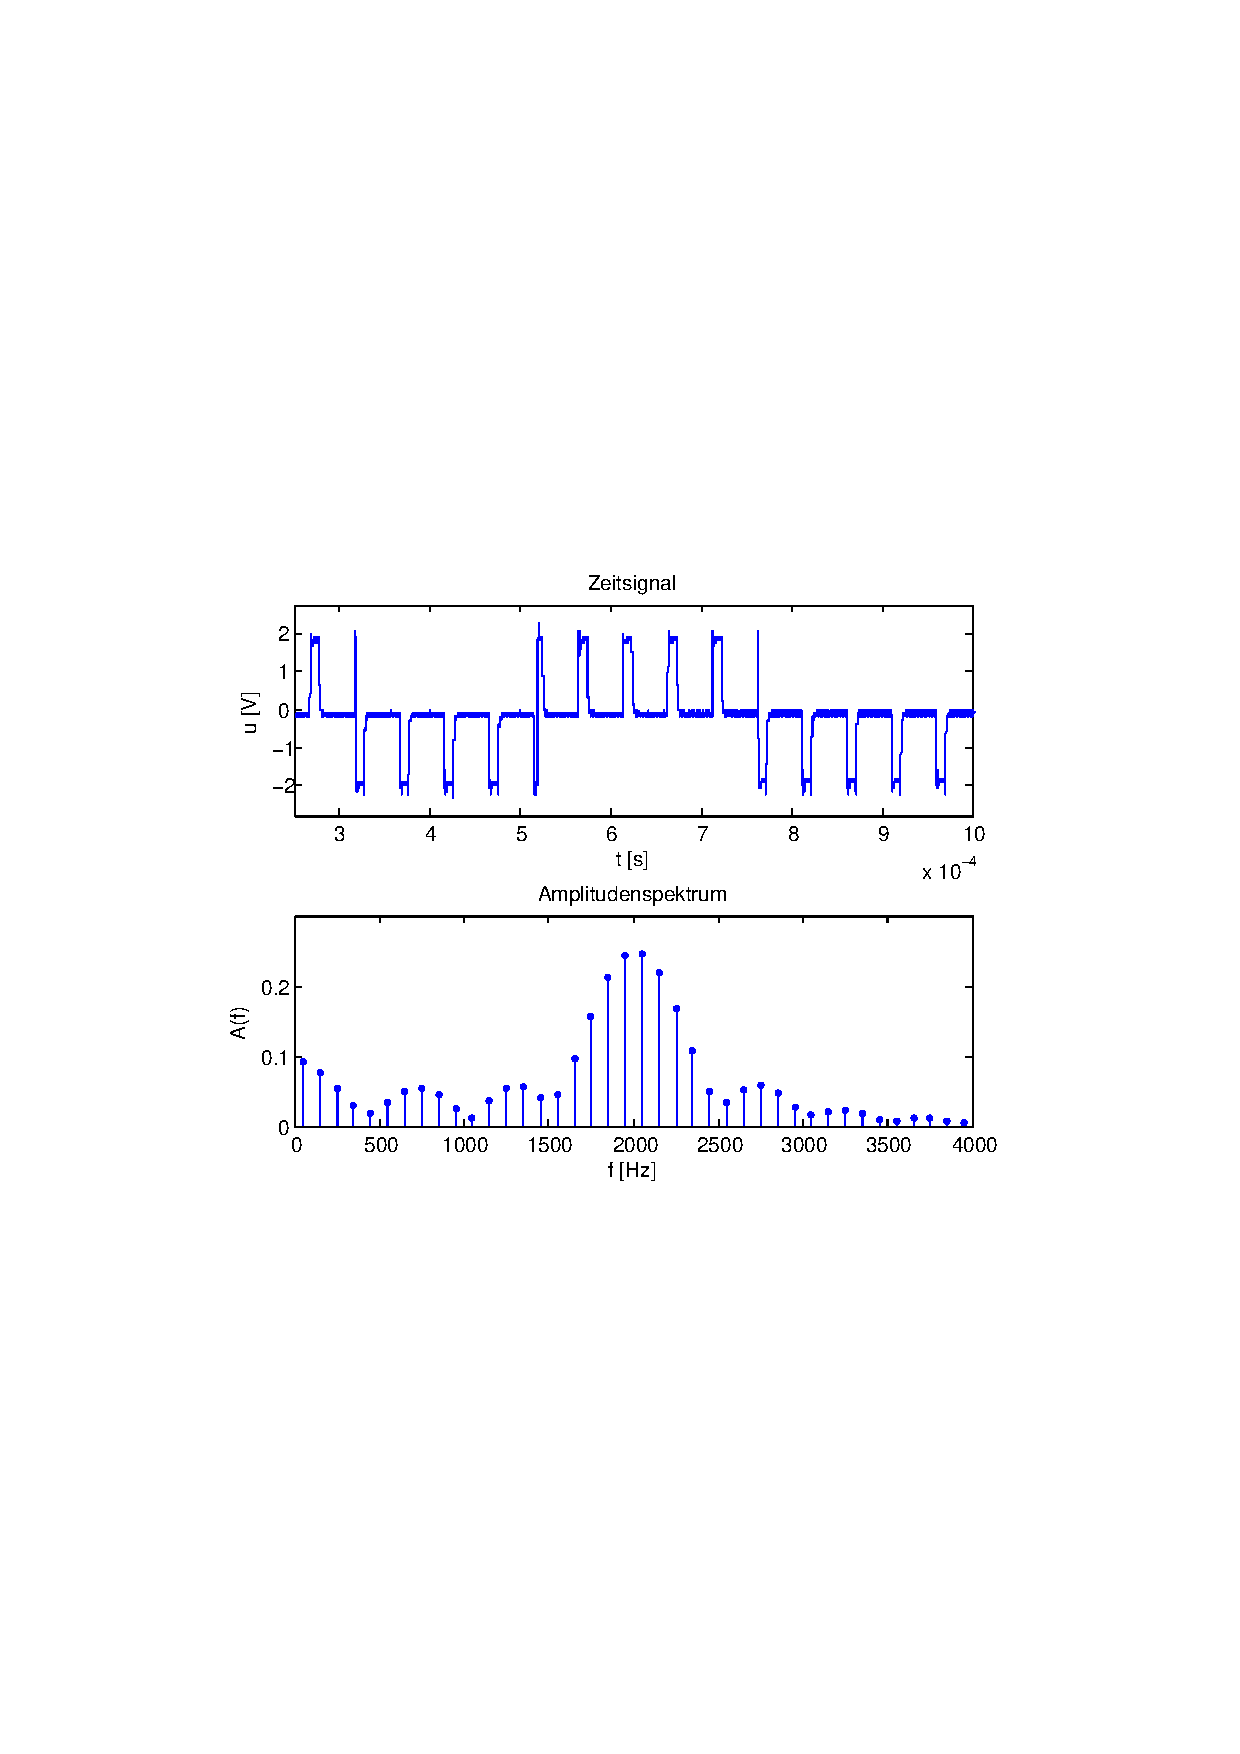
\includegraphics[scale=0.7, trim = 35mm 100mm 35mm 95mm, clip]{Bilder/flatrec20_02abget_zeit}
                          \caption{Rechteck 20 kHz alpha 0,2 moduliertes Signal}
		                  \label{fig:flatrec20_02zeit}
                    \end{figure}
                \end{minipage}
                
                \begin{minipage}{0.6\textwidth}
                    \begin{figure}[H]
                        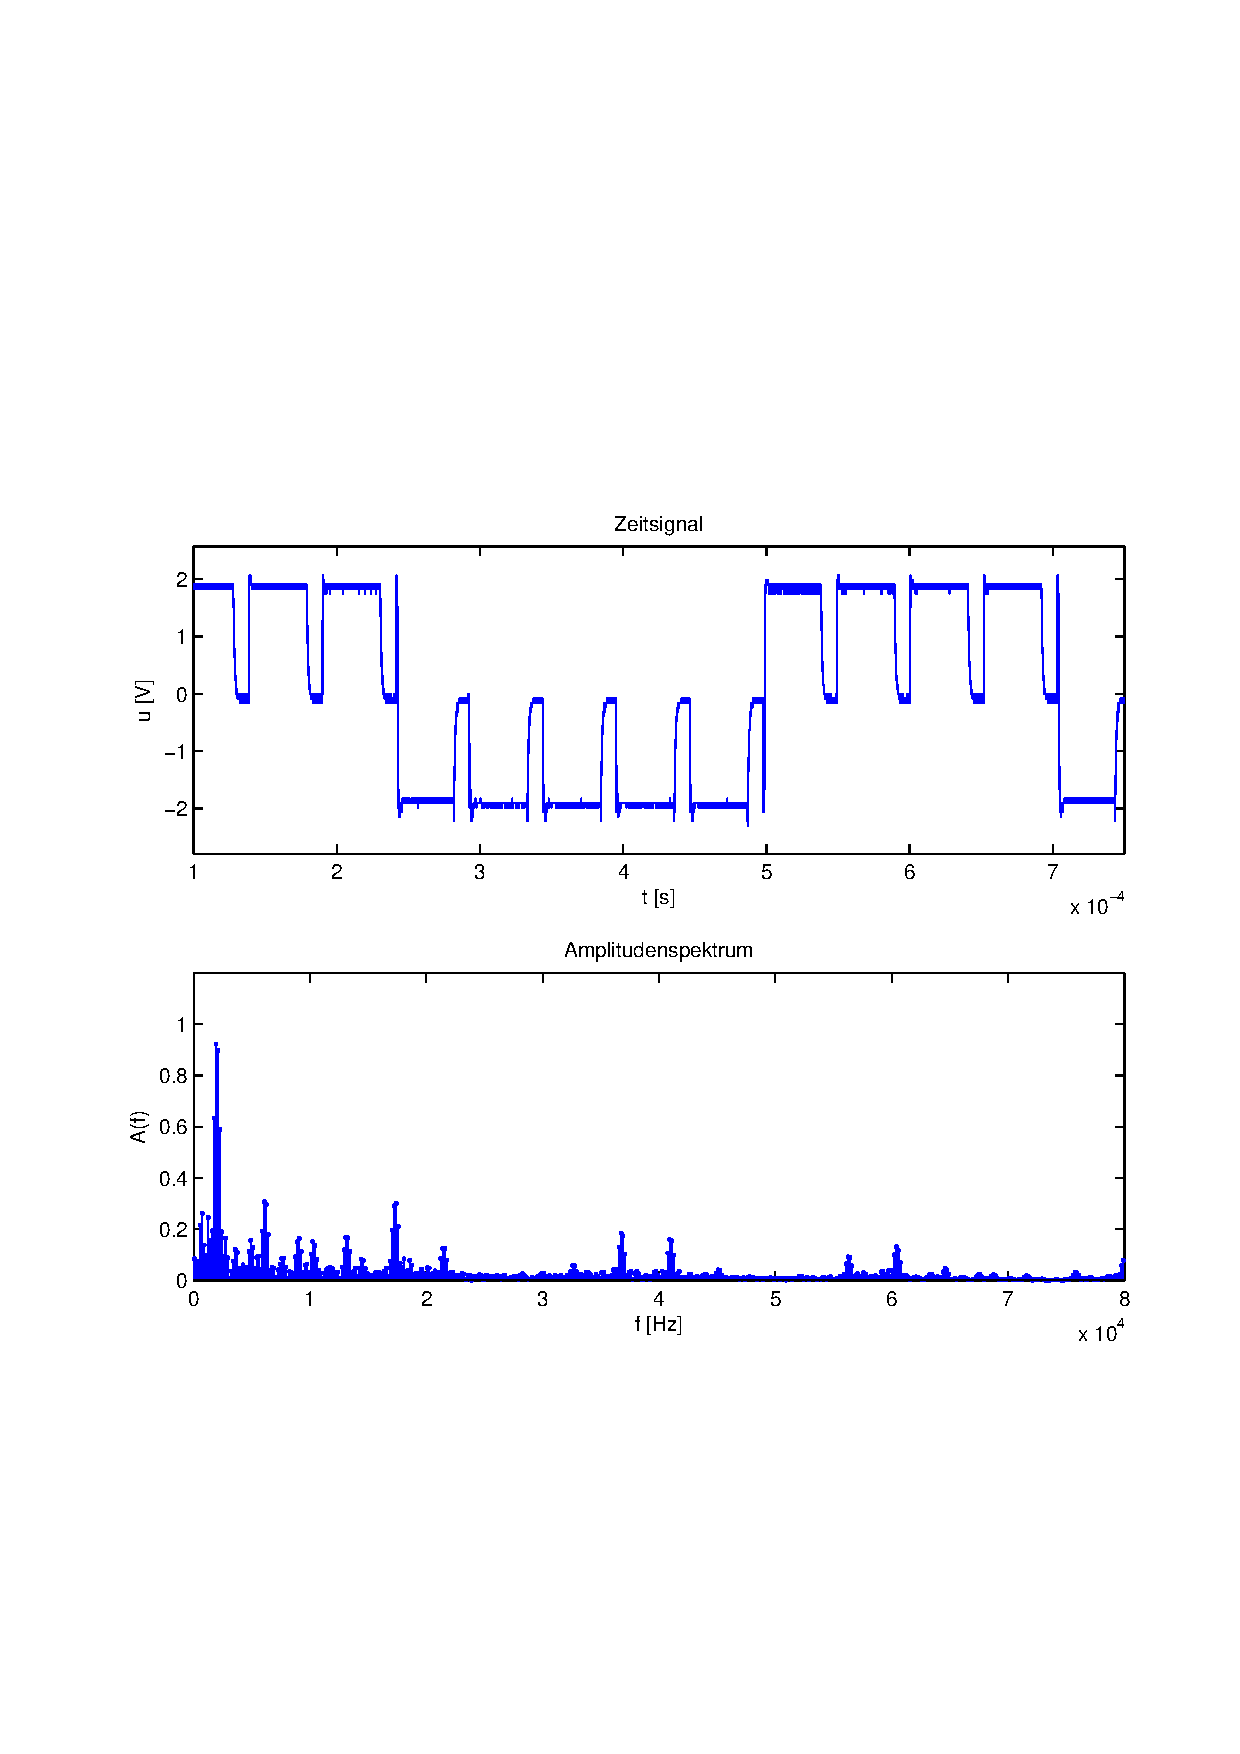
\includegraphics[scale=0.7, trim = 35mm 100mm 35mm 95mm, clip]{Bilder/flatrec20_07abget_zeit}
                       \caption{Rechteck 20 kHz alpha 0,7 moduliertes Signal}
		              \label{fig:flatrec20_07zeit}
                    \end{figure}
                \end{minipage}
            
            \end{tabular}
            \end{center}
            
            \begin{center}
            \begin{tabular}{ll}
            
            \hspace{-5cm}
                \begin{minipage}{0.6\textwidth}
                    \begin{figure}[H]
                        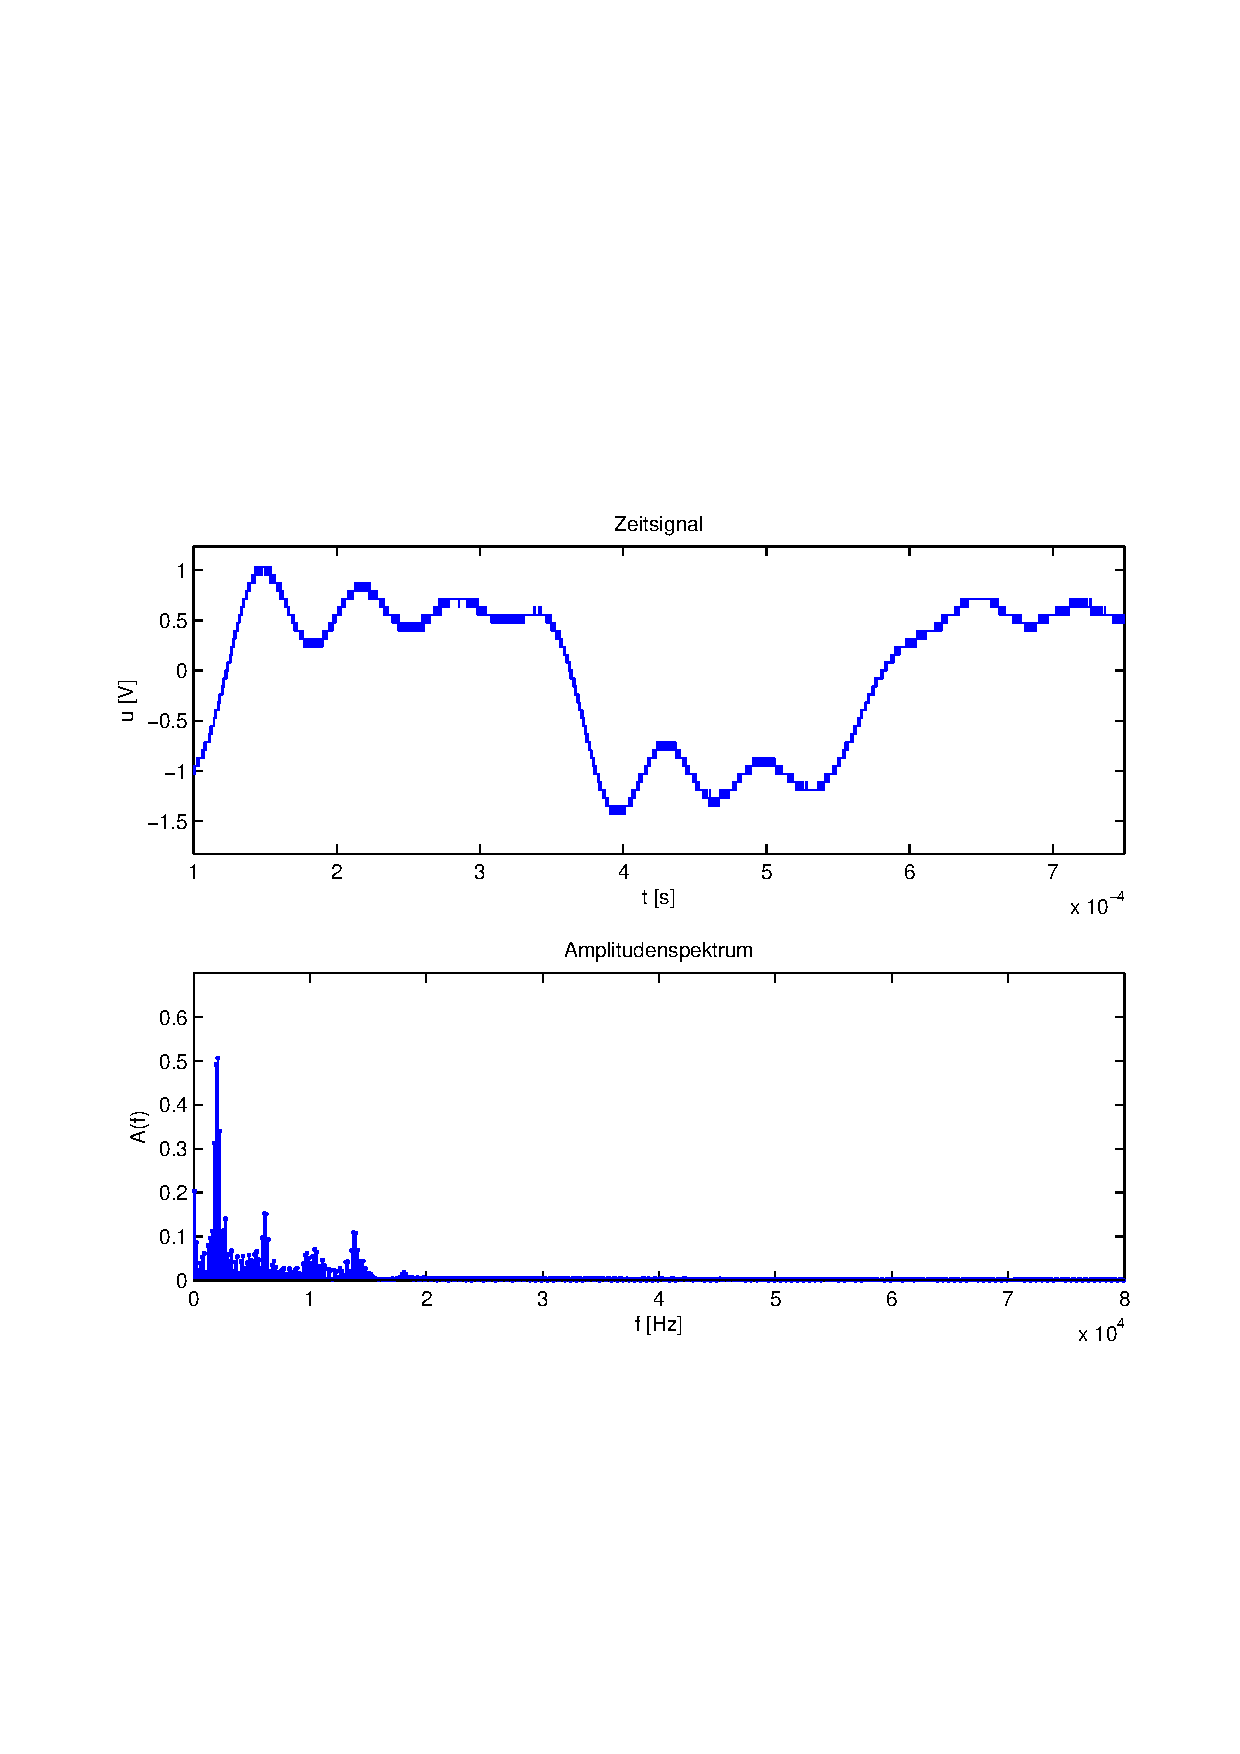
\includegraphics[scale=0.7, trim = 35mm 100mm 35mm 95mm, clip]{Bilder/flatrec20_02}
                          \caption{Rechteck 20 kHz alpha 0,2 Rekonstruktion}
		                  \label{fig:flatrec20_02}
                    \end{figure}
                \end{minipage}
                
                \begin{minipage}{0.6\textwidth}
                    \begin{figure}[H]
                        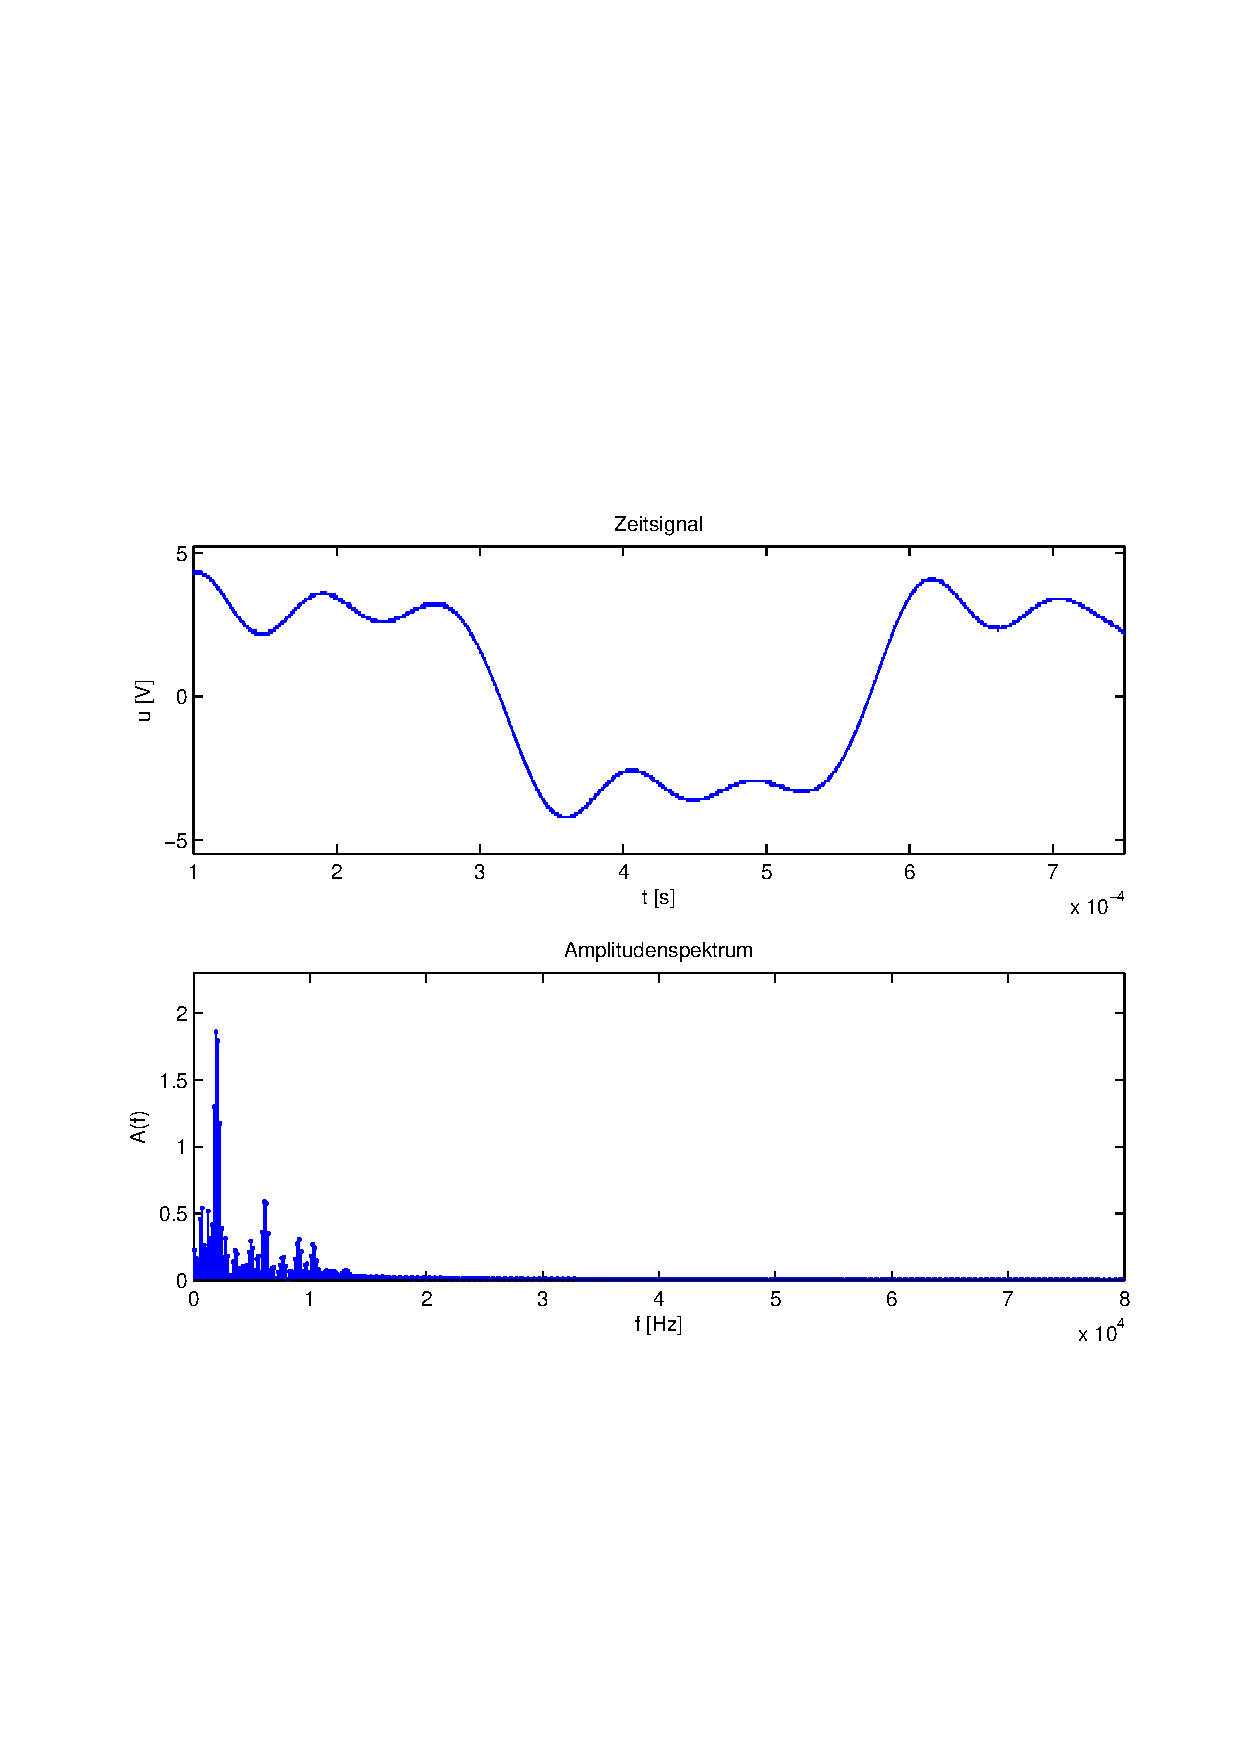
\includegraphics[scale=0.7, trim = 35mm 100mm 35mm 95mm, clip]{Bilder/flatrec20_07}
                       \caption{Rechteck 20 kHz alpha 0,7 Rekonstruktion}
		              \label{fig:flatrec20_07}
                    \end{figure}
                \end{minipage}
            
            \end{tabular}
            \end{center}
             
            Wie schon bei $\alpha=0,5$ haben die Spektren des modulierten Signals in Abb. \ref{fig:flatrec20_05} und
            \ref{fig:flatrec10_05} und des rekonstruierten Signals (was dem Ausgangssignal entsprechen soll) Abb. \ref{fig:flatrec10_05zeit} und
            \ref{fig:flatrec20_05zeit} in der Amplitude annähernd den Faktor 0,5 Unterschied, was dem $\alpha$
            aus der Formel \ref{eq:flat} als Faktor zwischen dem Spektrm des modulierten Signals und des
            Ausgangssignals entspricht.
                        
             
        \end{quote}
    
    \end{quote}
    
    \subsection{Shape-Top Sampling}
    \begin{quote}
        
        
        \subsubsection{Änderung der Trägerfrequenz}
        \begin{quote}
            
            Auch bei der Shape-Top Abtastung sollte aus der Vergrößerung der Trägerfrequenz eine bessere
            Rekonstruktion resultieren.
            
            \begin{center}
            \begin{tabular}{ll}
            
            \hspace{-5cm}
                \begin{minipage}{0.6\textwidth}
                    \begin{figure}[H]
                        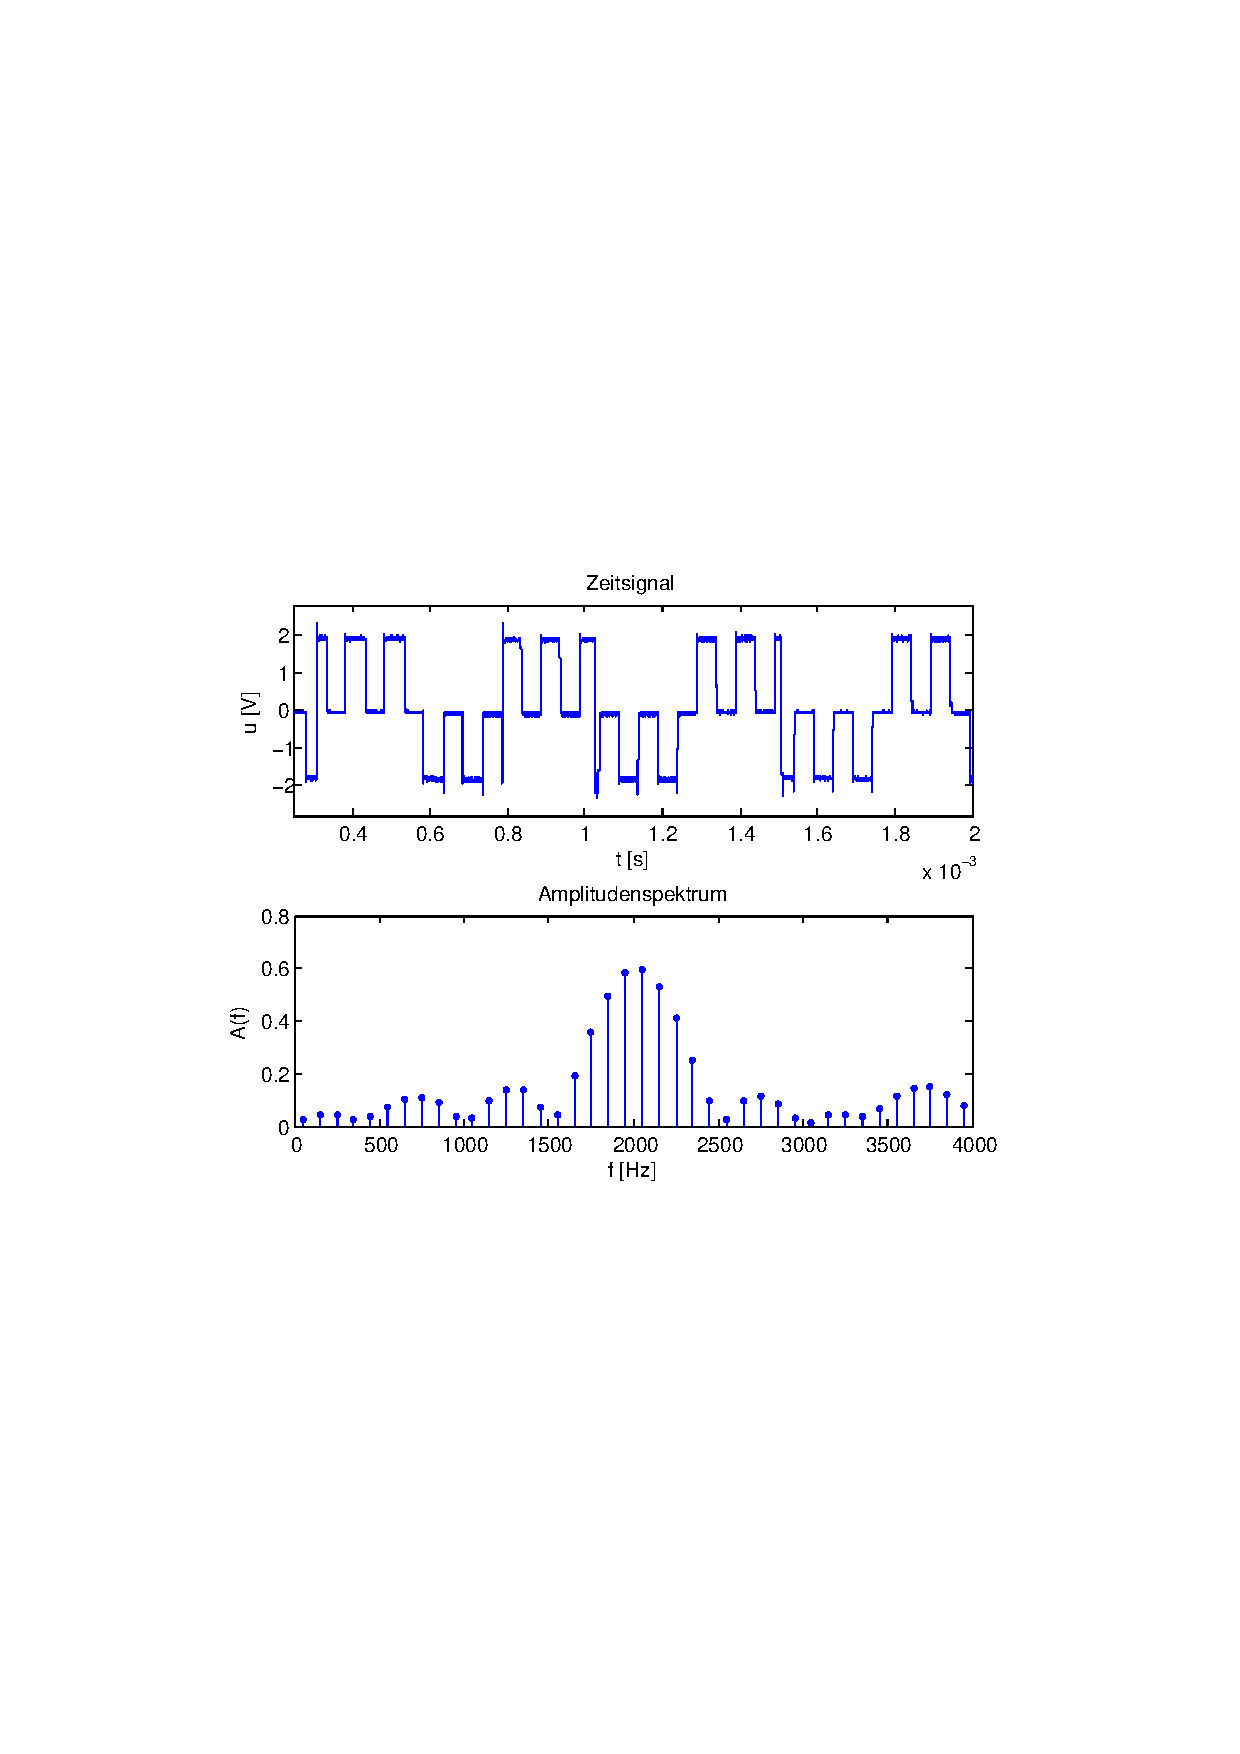
\includegraphics[scale=0.7, trim = 35mm 100mm 35mm 95mm, clip]{Bilder/shaperec10_05abget_zeit}
                          \caption{Rechteck 10 kHz alpha 0,5 moduliertes Signal}
		                  \label{fig:shaperec10_05zeit}
                    \end{figure}
                \end{minipage}
                
                \begin{minipage}{0.6\textwidth}
                    \begin{figure}[H]
                        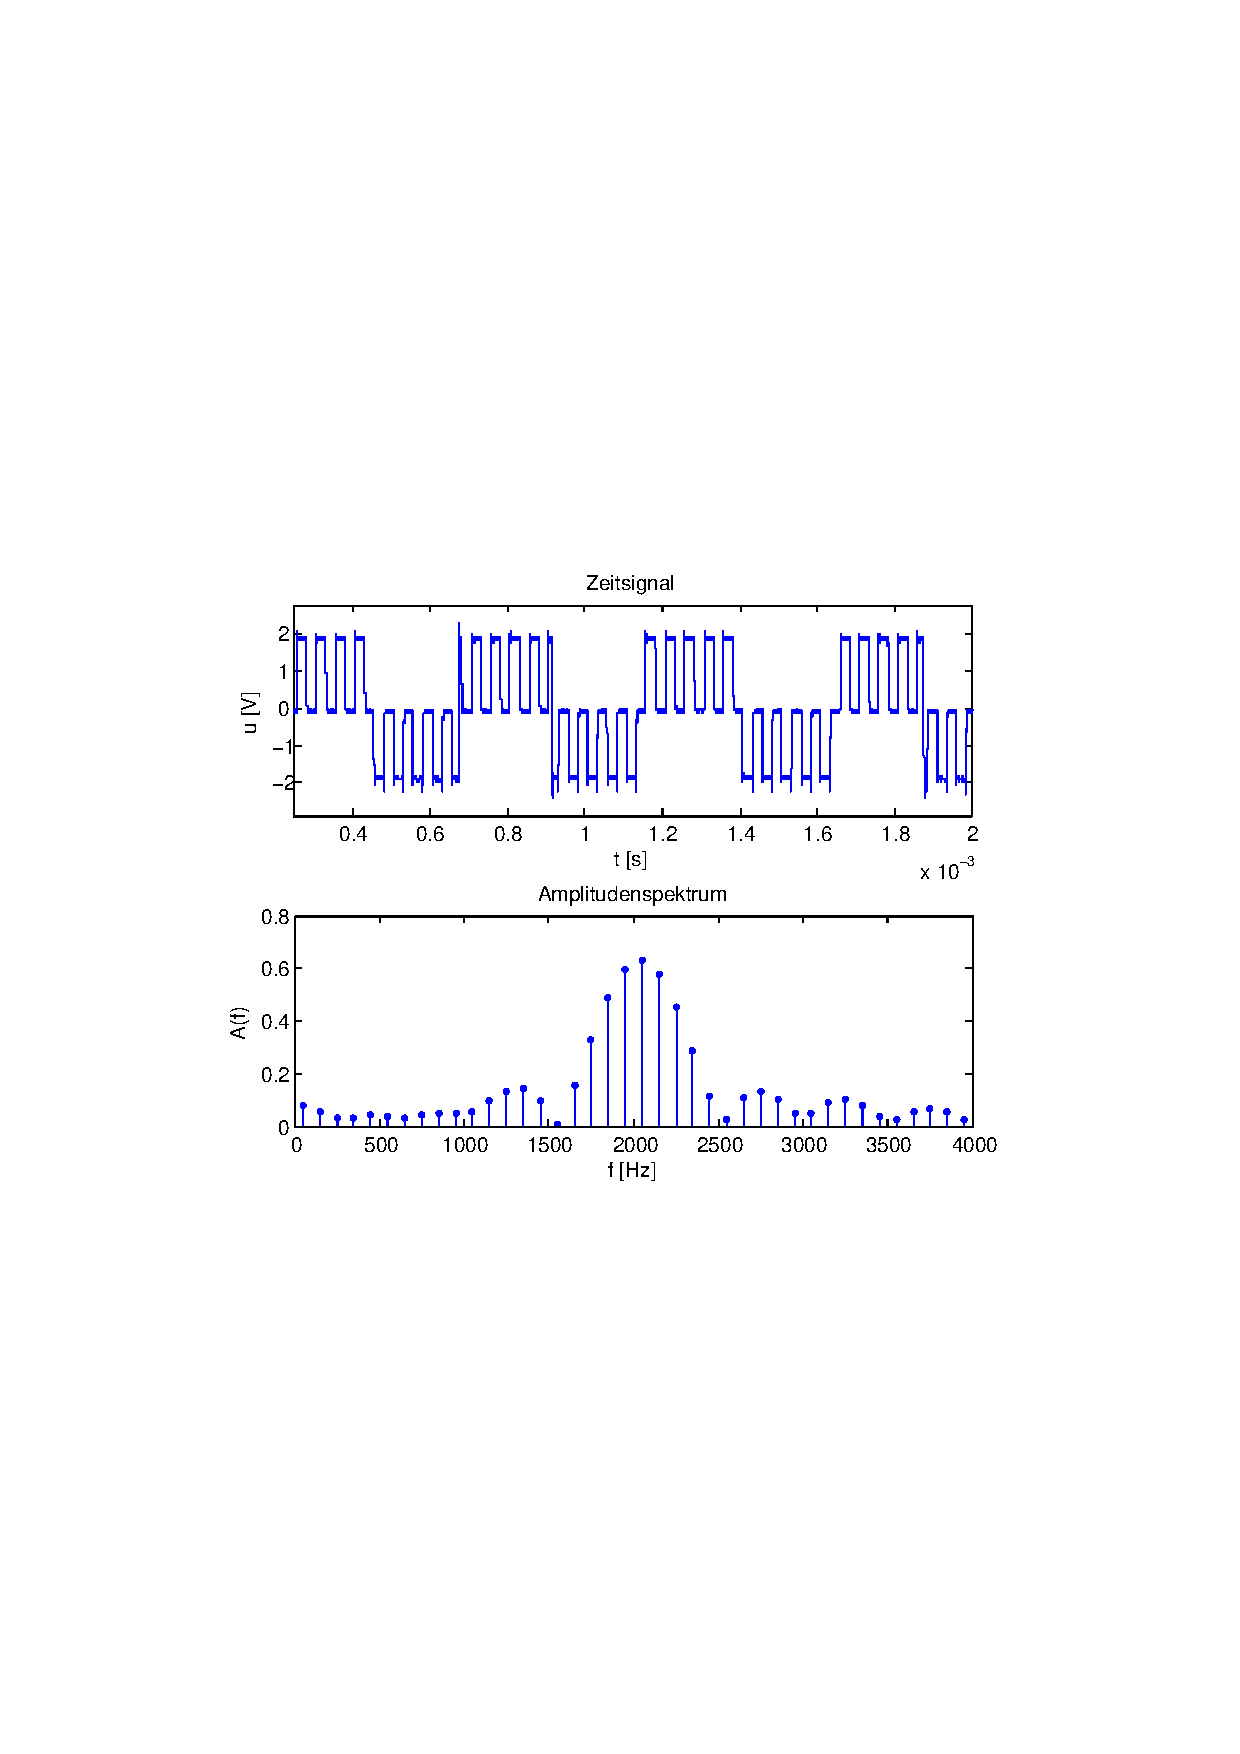
\includegraphics[scale=0.7, trim = 35mm 100mm 35mm 95mm, clip]{Bilder/shaperec20_05abget_zeit}
                       \caption{Rechteck 20 kHz alpha 0,5 moduliertes Signal}
		              \label{fig:shaperec20_05zeit}
                    \end{figure}
                \end{minipage}
            
            \end{tabular}
            \end{center}
            
            \begin{center}
            \begin{tabular}{ll}
            
            \hspace{-5cm}
                \begin{minipage}{0.6\textwidth}
                    \begin{figure}[H]
                        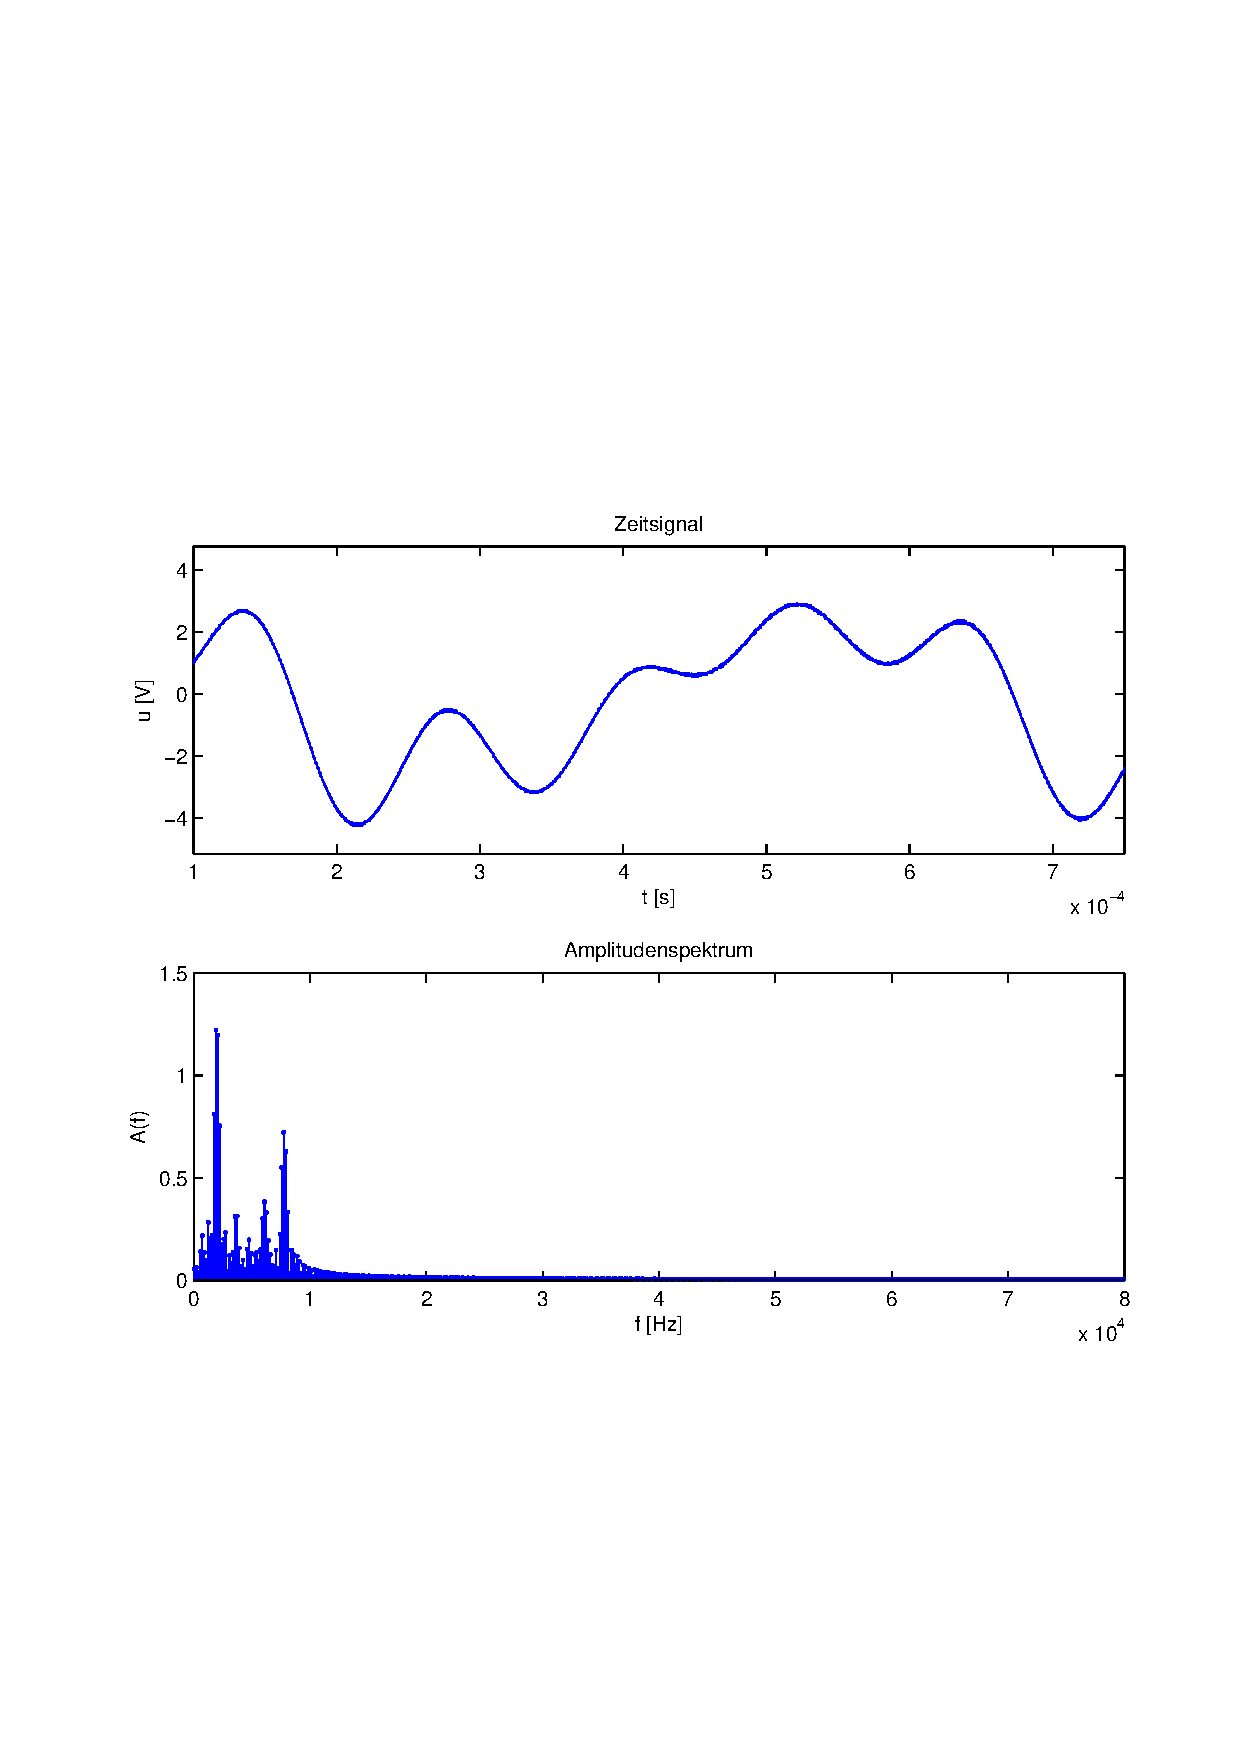
\includegraphics[scale=0.7, trim = 35mm 100mm 35mm 95mm, clip]{Bilder/shaperec10_05}
                          \caption{Rechteck 10 kHz alpha 0,5 Rekonstruktion}
		                  \label{fig:shaperec10_05}
                    \end{figure}
                \end{minipage}
                
                \begin{minipage}{0.6\textwidth}
                    \begin{figure}[H]
                        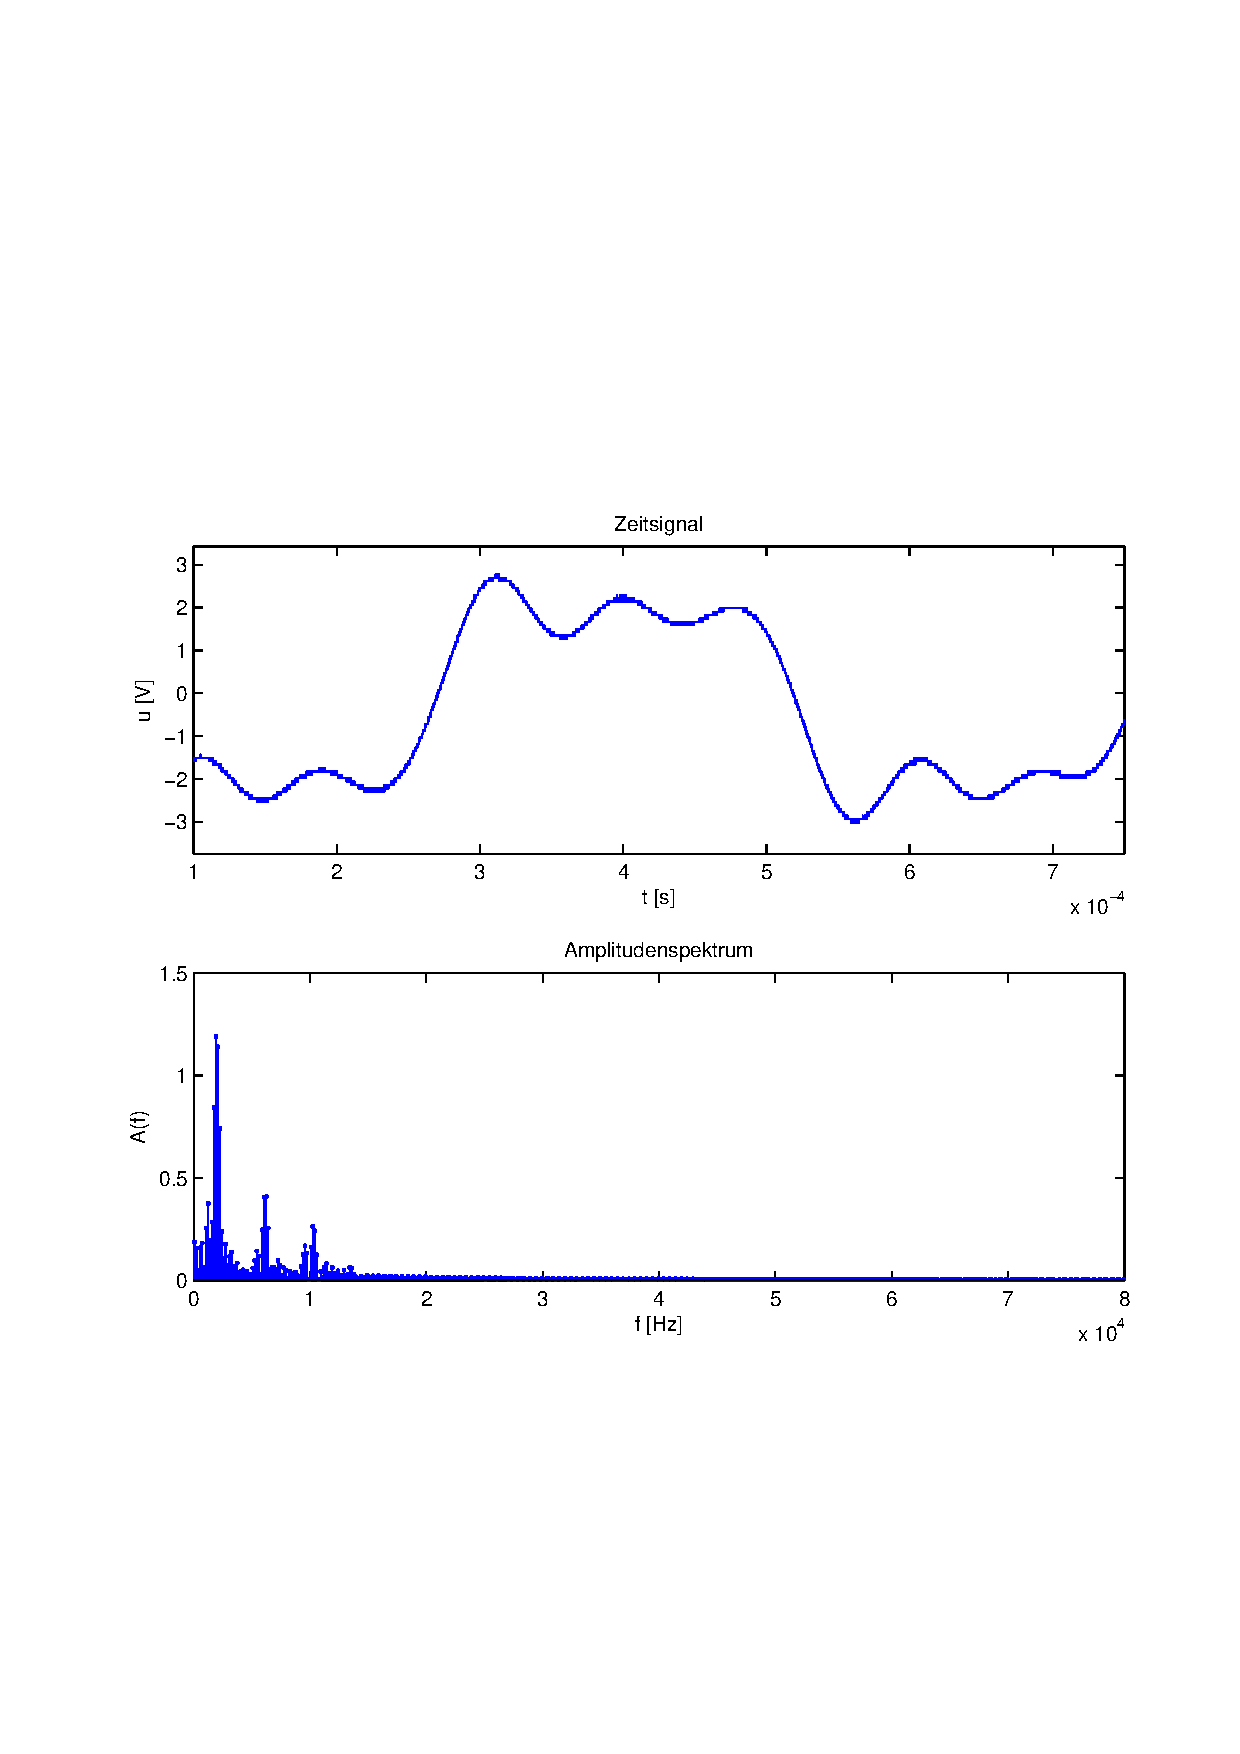
\includegraphics[scale=0.7, trim = 35mm 100mm 35mm 95mm, clip]{Bilder/shaperec20_05}
                       \caption{Rechteck 20 kHz alpha 0,5 Rekonstruktion}
		              \label{fig:shaperec20_05}
                    \end{figure}
                \end{minipage}
            
            \end{tabular}
            \end{center}
            
        \end{quote}
        
        In den Abb. \ref{fig:shaperec10_05} und \ref{fig:shaperec20_05} ist der Unterschied der Rekonstruktion zwischen
        10 und 20 kHz Signalausblendung noch deutlicher zu erkennen als bei der Signalverbreiterung.
        
        \TODO{Was kann man da noch erkennen????}
        
        \subsubsection{Änderung des Tastgrades}
        \begin{quote}
            
                      
             Im Gegensatz zur Signalverbreiterung sollte sich bei der Signalausblendung das Basisband (k=0) nur um den
             Faktor $\alpha$ verringern.
             Alle anderen Bänder sollten sich noch zusätzlich um den Faktor $si(k\alpha\pi)$ verringern%, was zu einer Verzerrung führt.
             % (gibt keine Verzerrung) ja stimmt, kann ich auch nicht wirklich erkennen, sollte aber eigentlich so sein,
             % kp skript seite 263 im pdf reader
             Dieses Verhalten zeigt sich in der Praxis (Abb. \ref{fig:shaperec} und \ref{fig:flatrec})wie auch schon
             in Skizze .\ref{fig:skizze}
             
             
             
             
            \begin{center}
            \begin{tabular}{ll}
            
            \hspace{-5cm}
                \begin{minipage}{0.6\textwidth}
                    \begin{figure}[H]
                        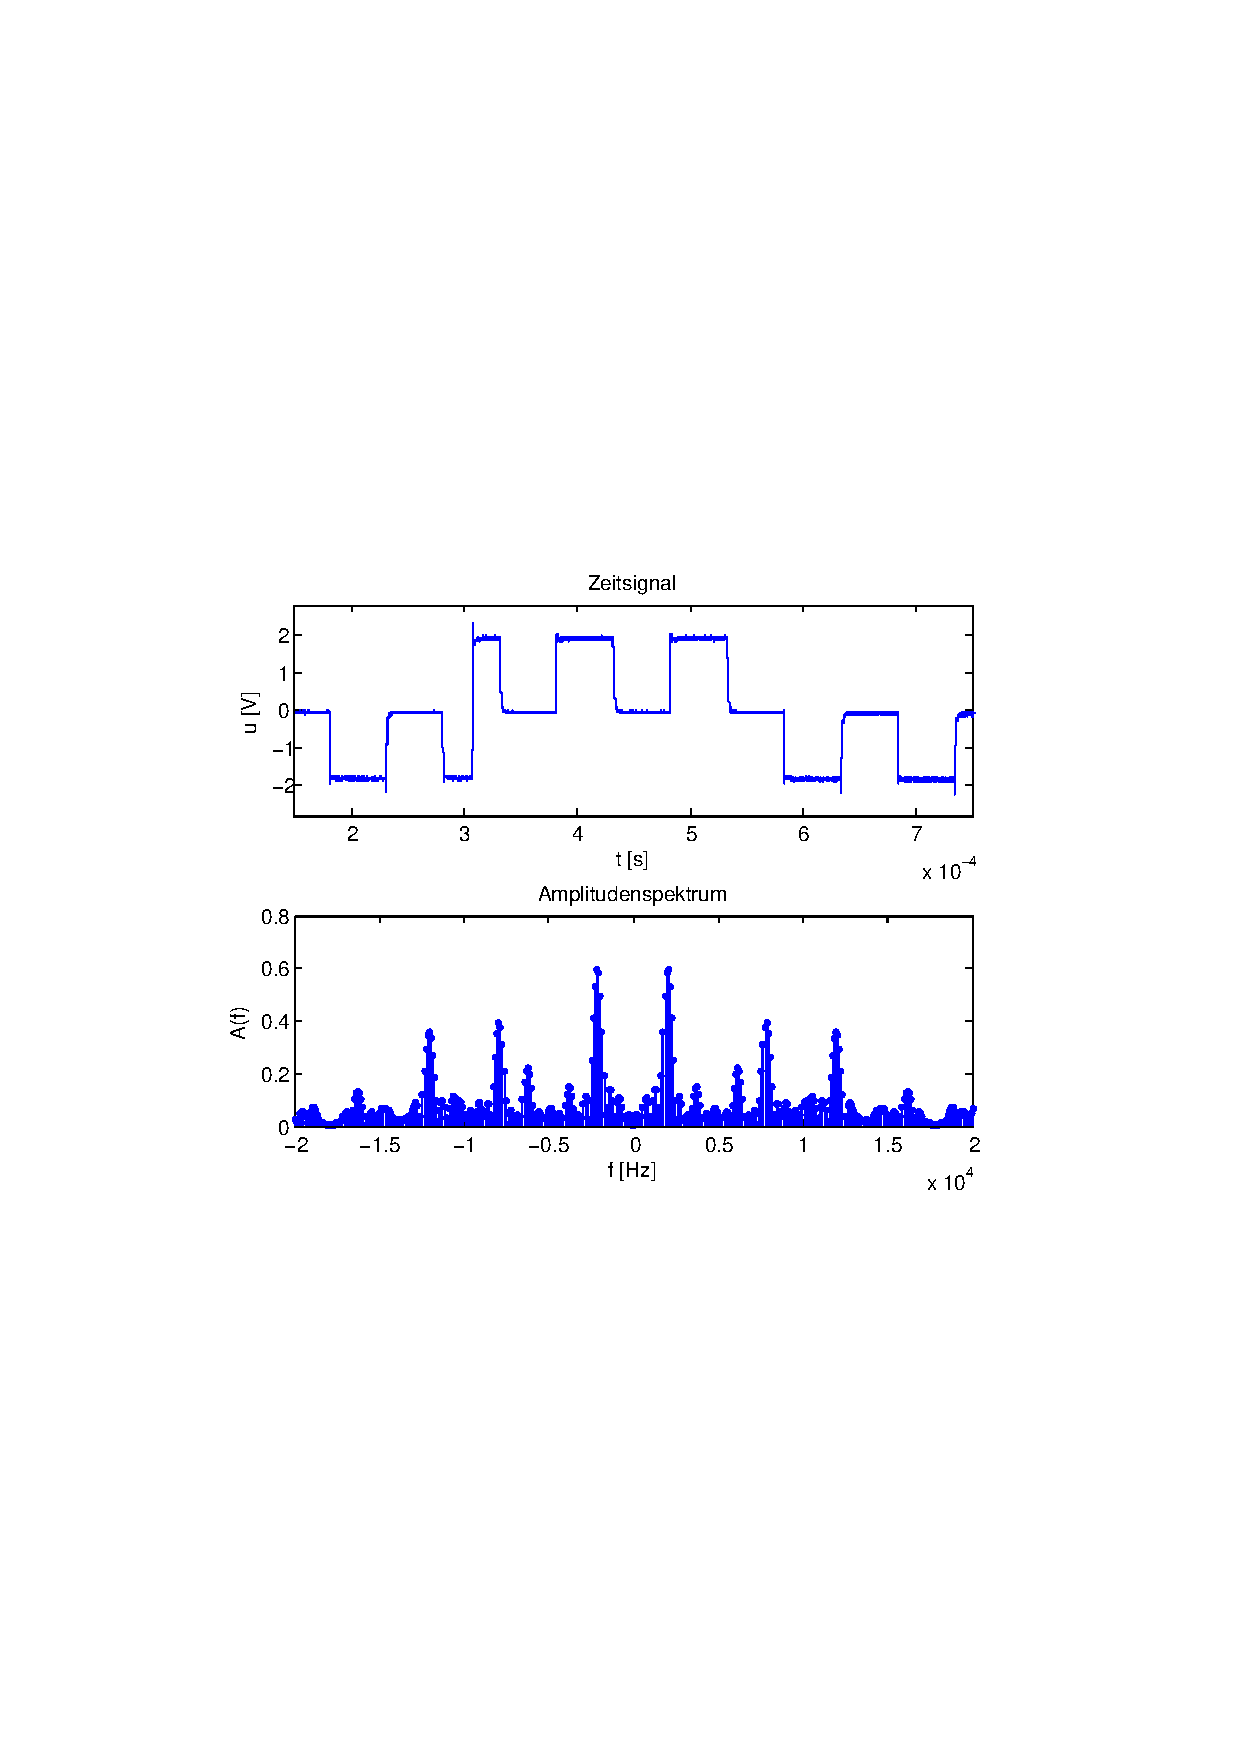
\includegraphics[scale=0.7, trim = 35mm 100mm 35mm 95mm, clip]{Bilder/shapeskizze}
                          \caption{Shape-Top-Sampling Rechteck}
		                  \label{fig:shaperec}
                    \end{figure}
                \end{minipage}
                
                \begin{minipage}{0.6\textwidth}
                    \begin{figure}[H]
                        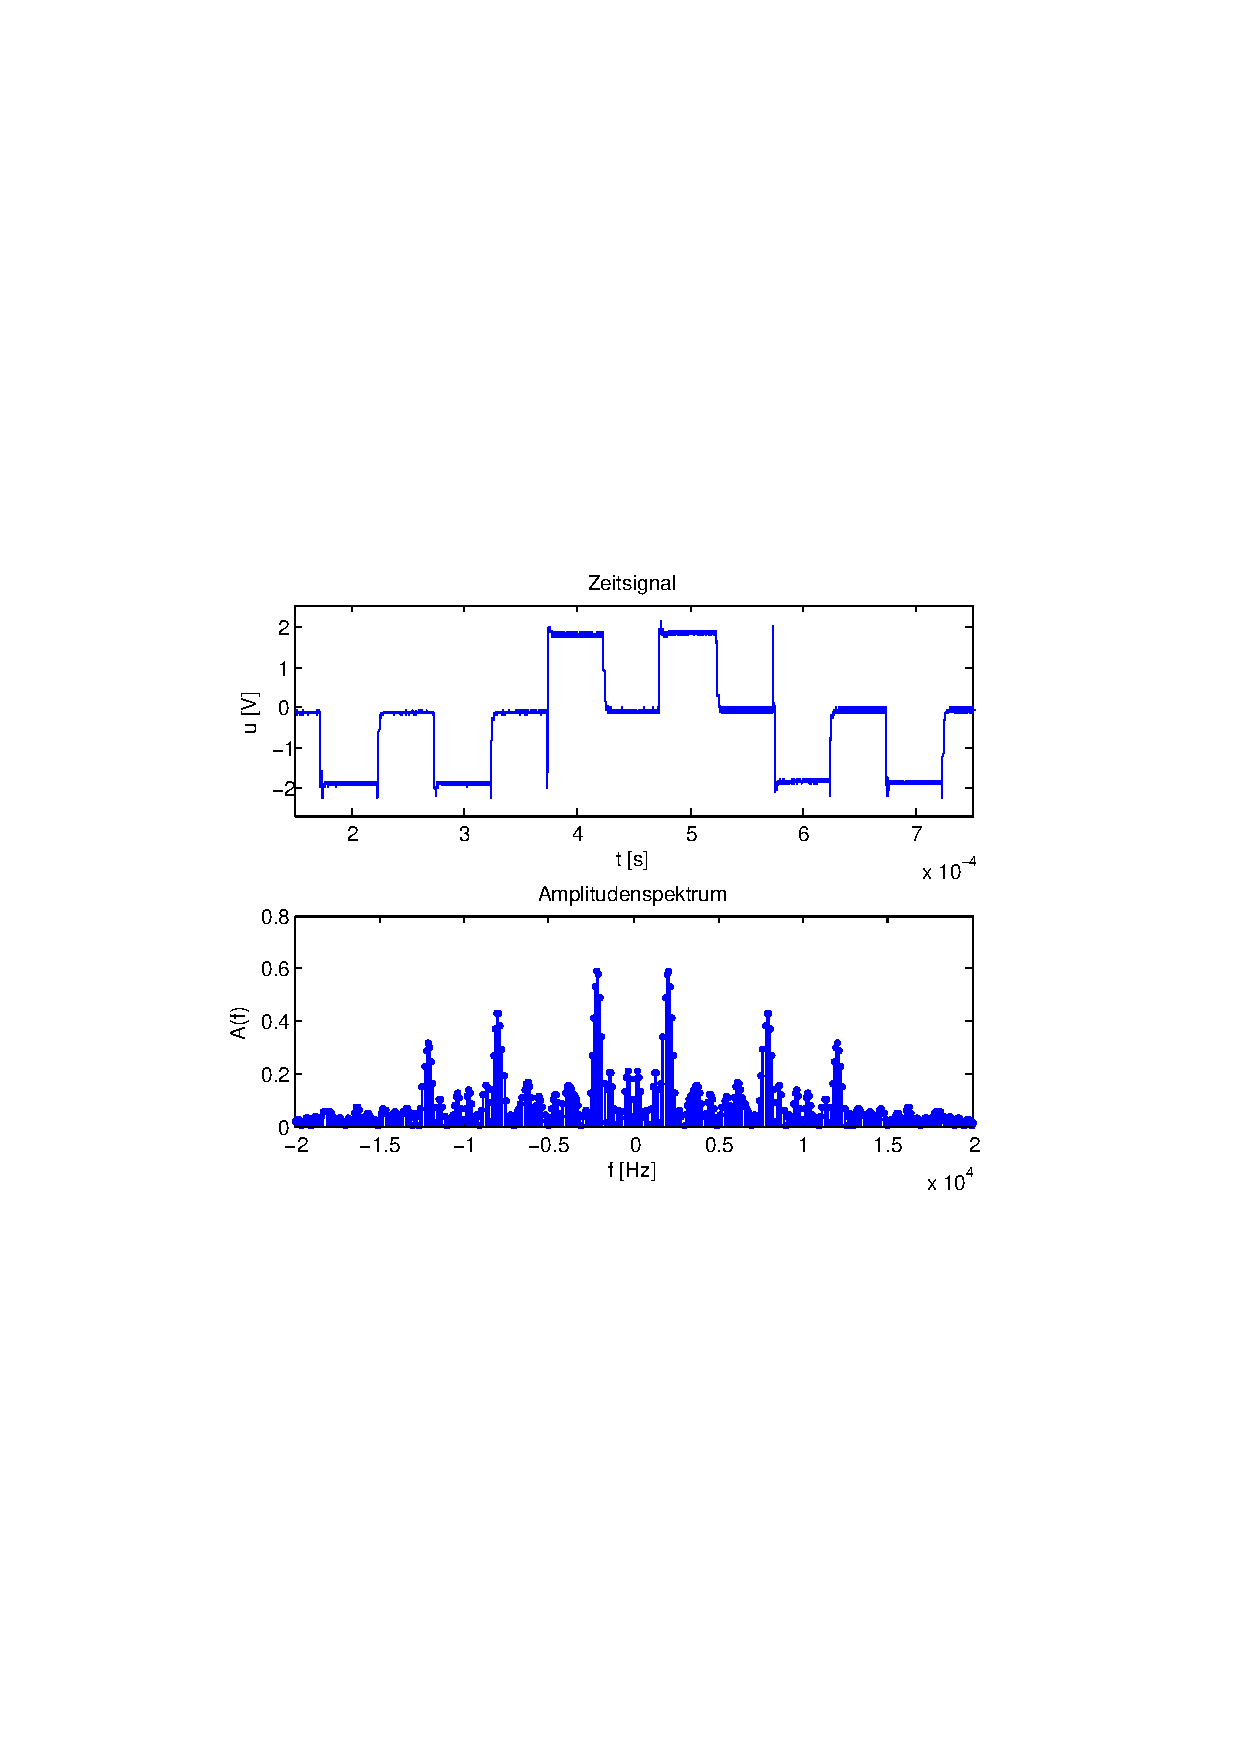
\includegraphics[scale=0.7, trim = 35mm 100mm 35mm 95mm, clip]{Bilder/flatskizze}
                       \caption{Flat-Top-Sampling Rechteck}
		              \label{fig:flatrec}
                    \end{figure}
                \end{minipage}
            
            \end{tabular}
            \end{center}
            
            Da bei der Signalverbreiterung die Amplituden im Spektrum von der Frequenz abhängen (Vorfaktor: $si(\omega
             \alpha T/2)$), haben die beiden Nebenpeaks jeweils eine andere Amplitude. Hingegen ist der Vorfaktor bei
             der Signalaublendung unabhängig von der Frequenz und damit haben die jeweils zueinander
             gehörenden Peaks die gleiche Amplitude.
             
    
    %\begin{figure}[H]
	%	\begin{center}
	%		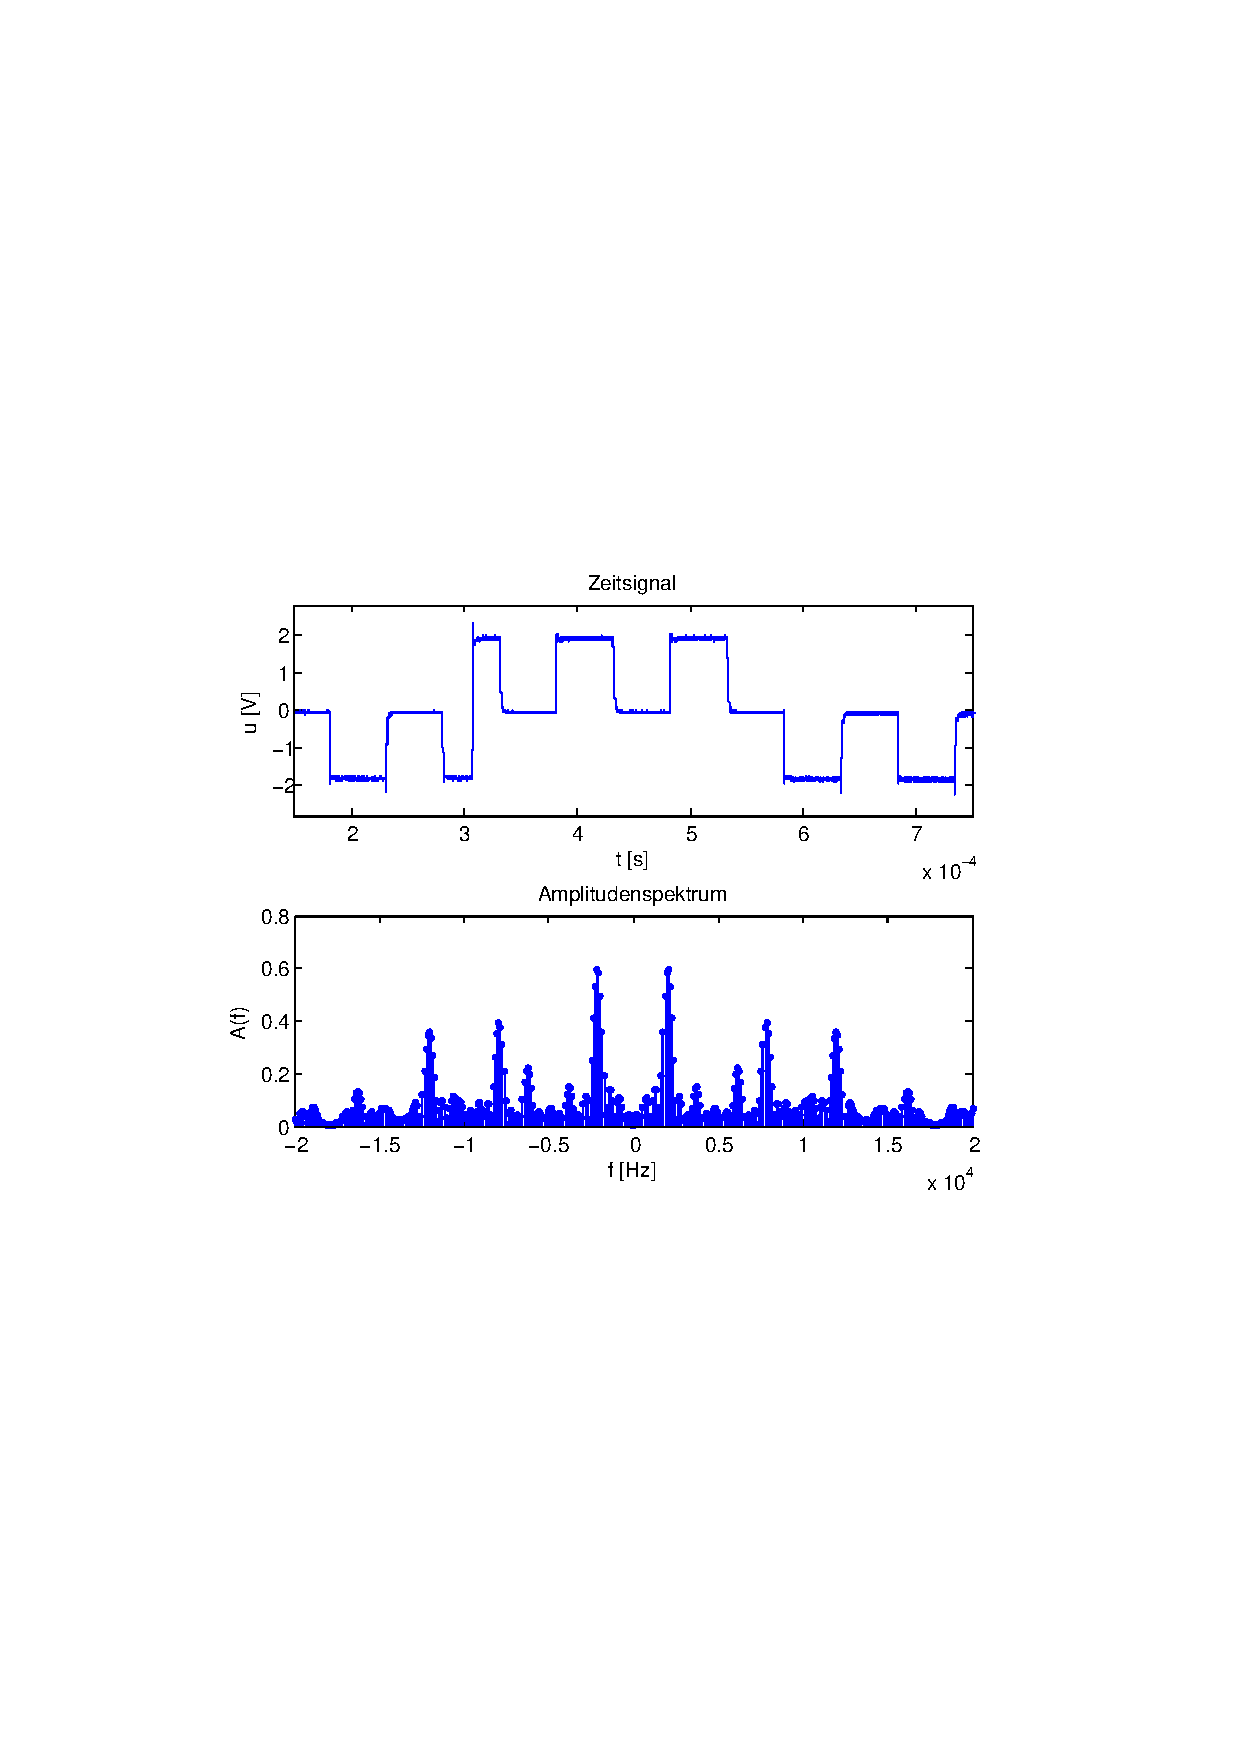
\includegraphics[scale=0.7, trim = 35mm 100mm 35mm 95mm, clip]{Bilder/shapeskizze}
	%	\end{center}
	%	\caption{Shape-Top-Sampling Rechteck}
	%	\label{fig:shaperec}
	%\end{figure}
             
             
             
             
             
             \begin{center}
            \begin{tabular}{ll}
            
            \hspace{-5cm}
                \begin{minipage}{0.6\textwidth}
                    \begin{figure}[H]
                        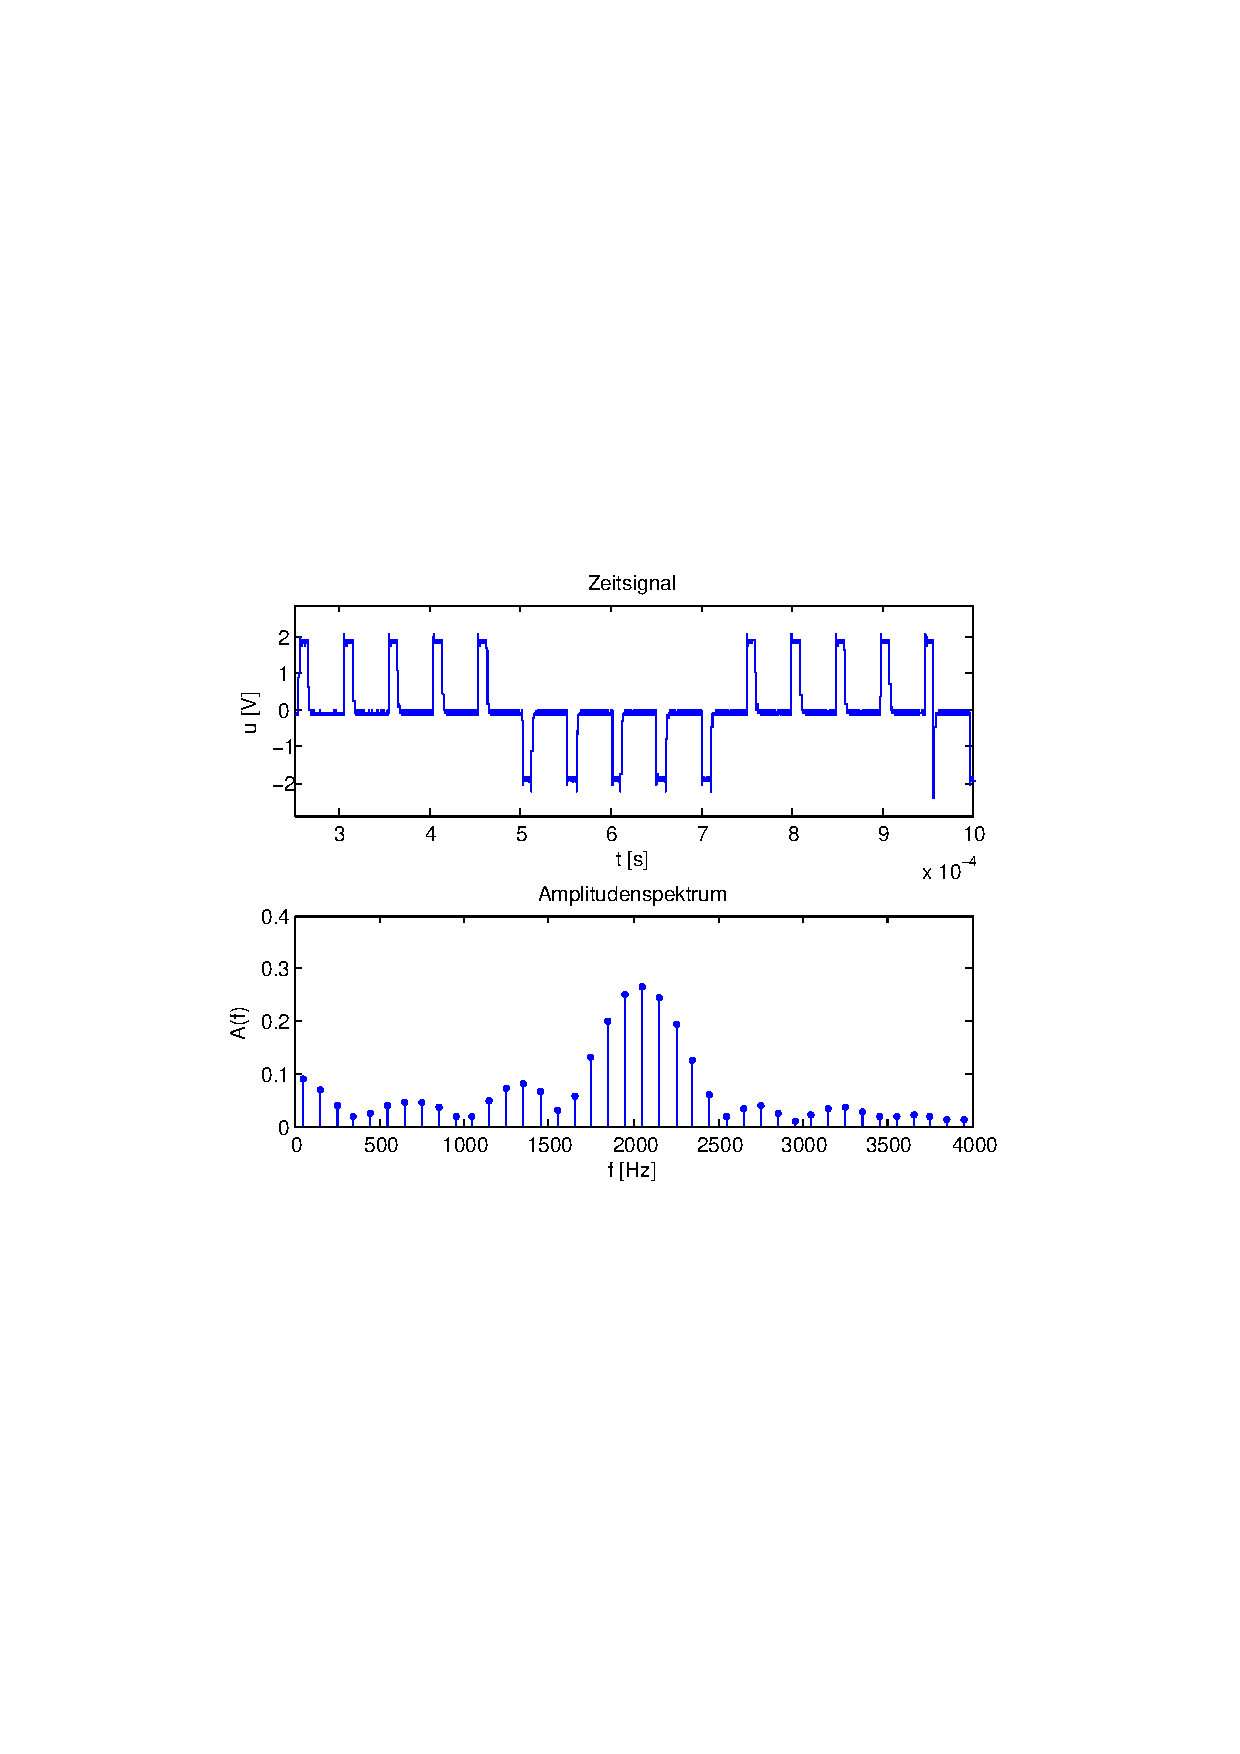
\includegraphics[scale=0.7, trim = 35mm 100mm 35mm 95mm, clip]{Bilder/shaperec20_02abget_zeit}
                          \caption{Rechteck 20 kHz alpha 0,2 moduliertes Signal}
		                  \label{fig:shaperec20_02zeit}
                    \end{figure}
                \end{minipage}
                
                \begin{minipage}{0.6\textwidth}
                    \begin{figure}[H]
                        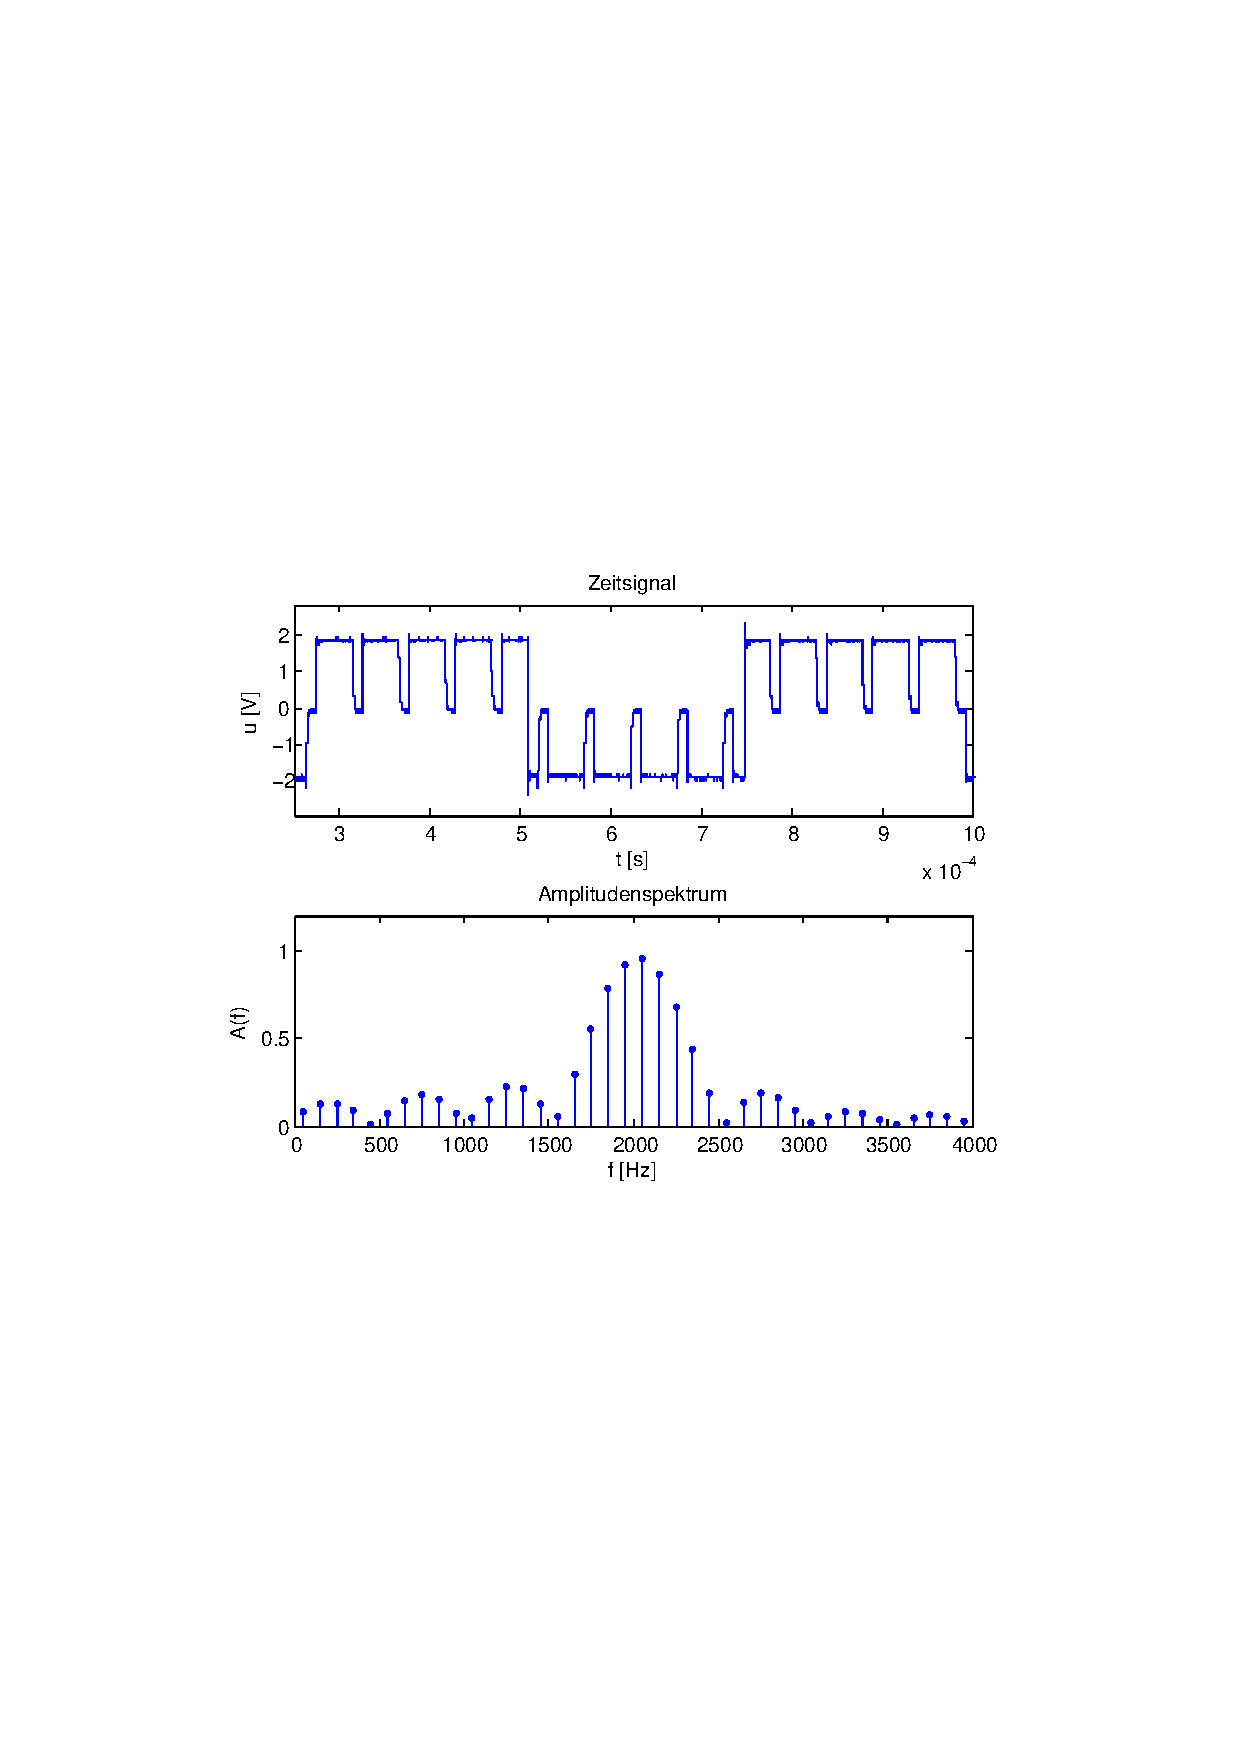
\includegraphics[scale=0.7, trim = 35mm 100mm 35mm 95mm, clip]{Bilder/shaperec20_07abget_zeit}
                       \caption{Rechteck 20 kHz alpha 0,7 moduliertes Signal}
		              \label{fig:shaperec20_07zeit}
                    \end{figure}
                \end{minipage}
            
            \end{tabular}
            \end{center}
            
            \begin{center}
            \begin{tabular}{ll}
            
            \hspace{-5cm}
                \begin{minipage}{0.6\textwidth}
                    \begin{figure}[H]
                        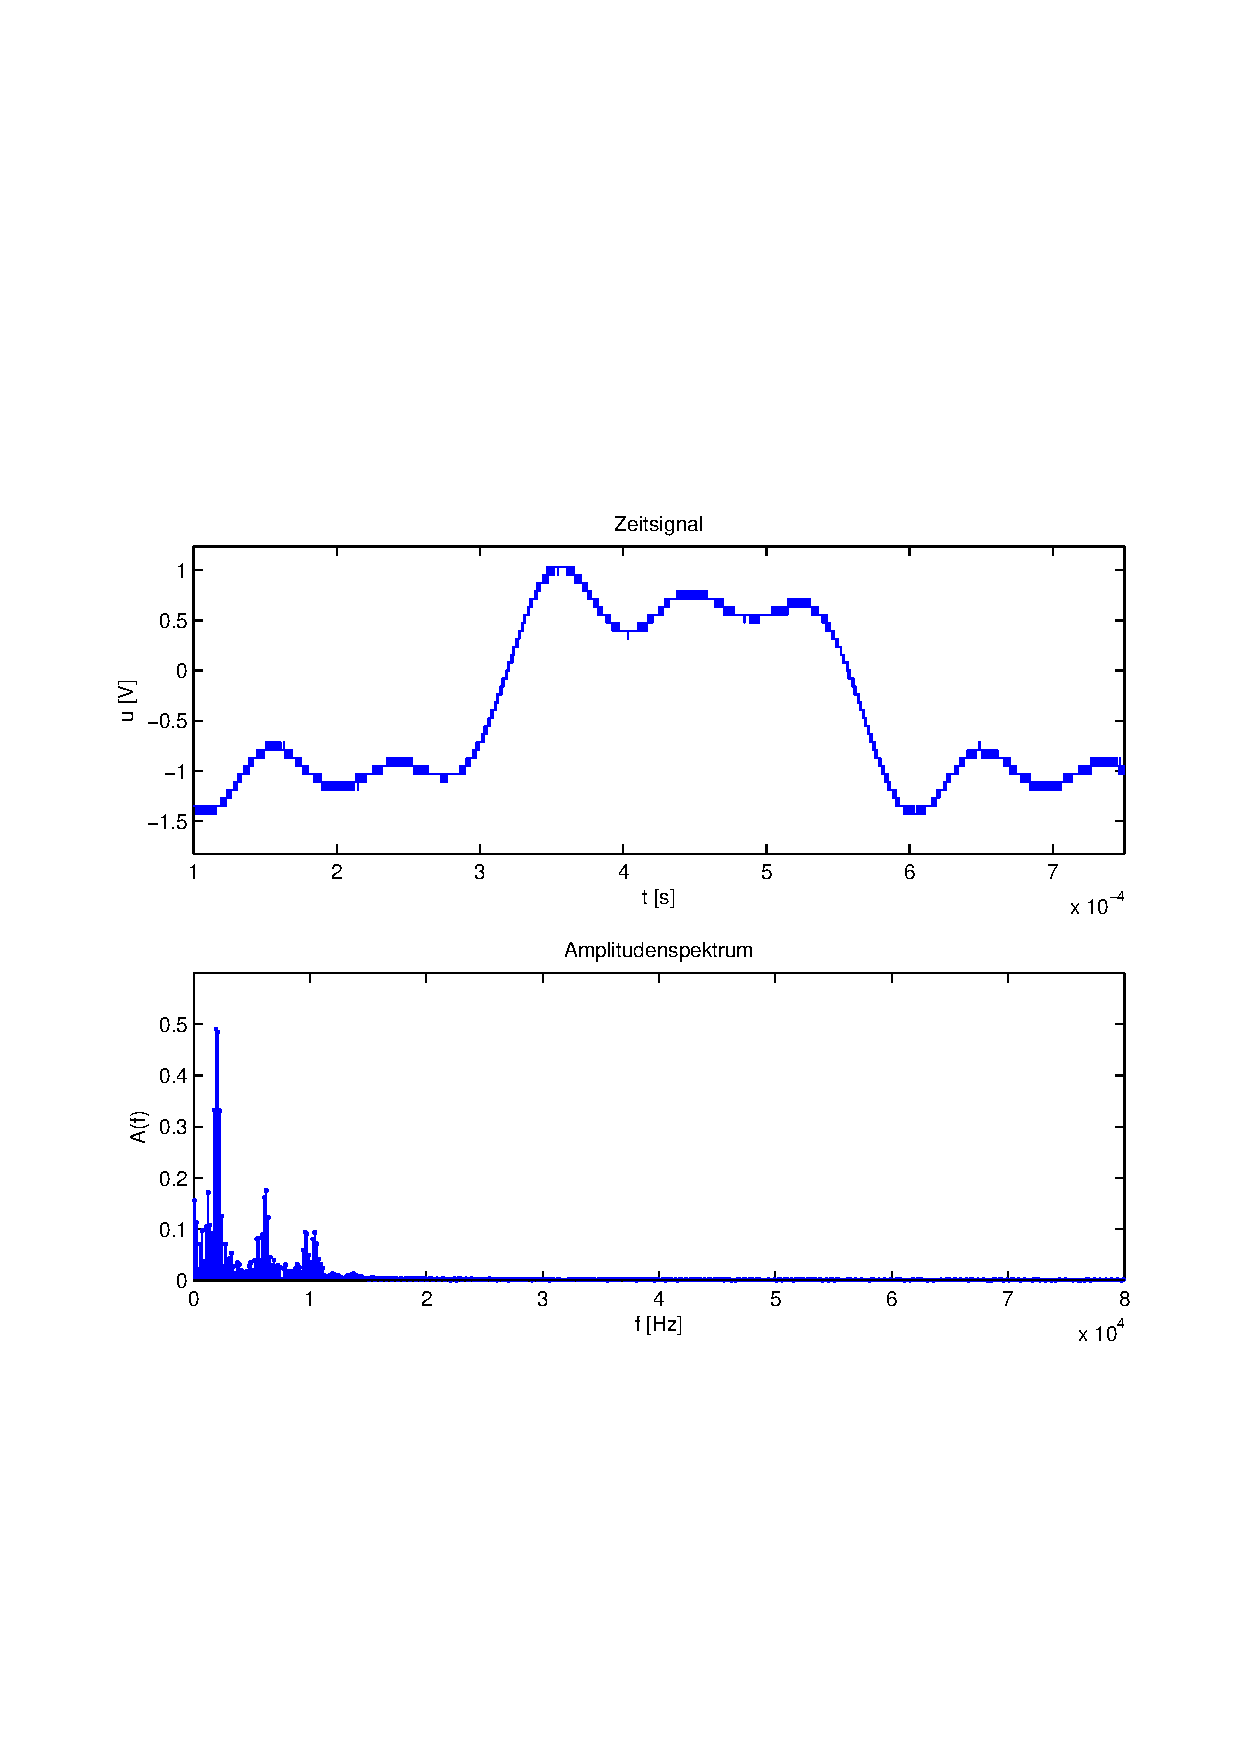
\includegraphics[scale=0.7, trim = 35mm 100mm 35mm 95mm, clip]{Bilder/shaperec20_02}
                          \caption{Rechteck 20 kHz alpha 0,2 Rekonstruktion}
		                  \label{fig:shaperec20_02}
                    \end{figure}
                \end{minipage}
                
                \begin{minipage}{0.6\textwidth}
                    \begin{figure}[H]
                        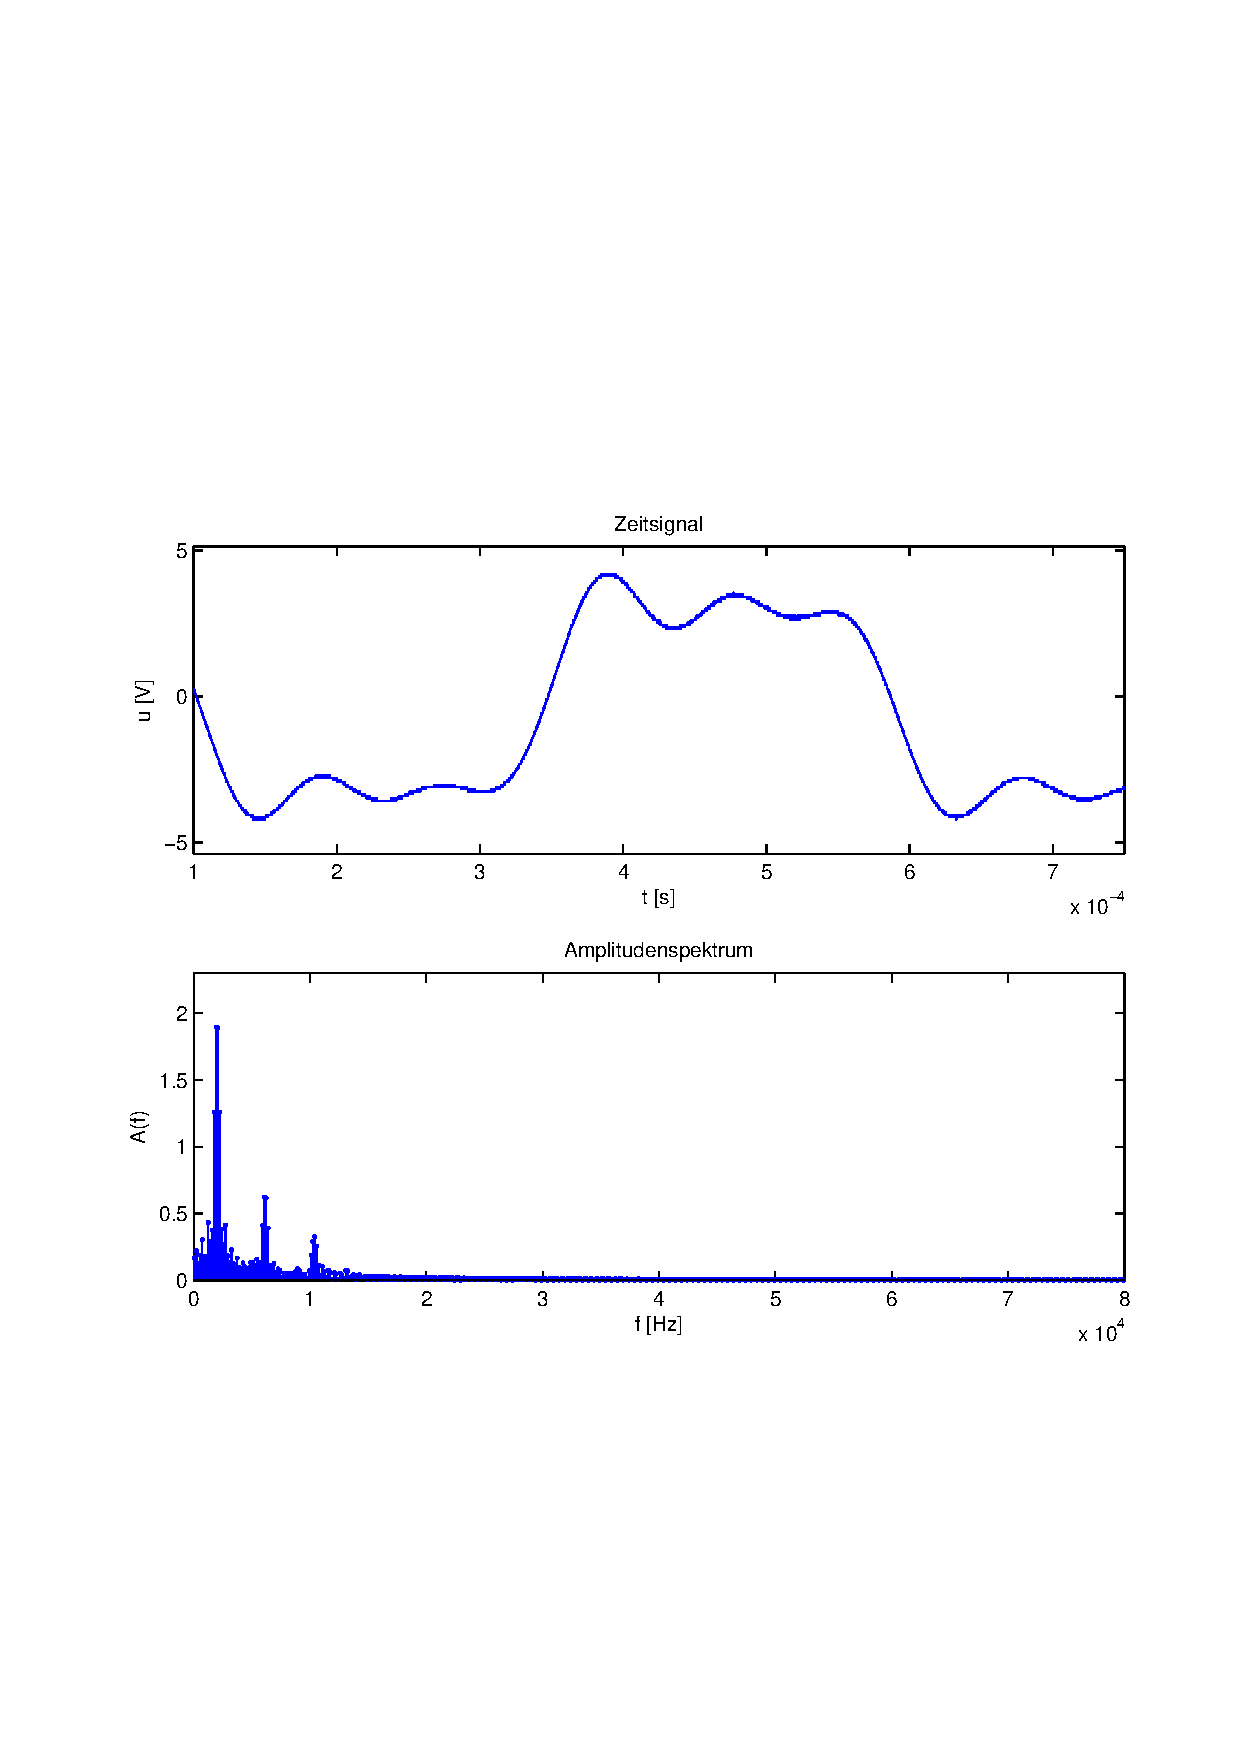
\includegraphics[scale=0.7, trim = 35mm 100mm 35mm 95mm, clip]{Bilder/shaperec20_07}
                       \caption{Rechteck 20 kHz alpha 0,7 Rekonstruktion}
		              \label{fig:shaperec20_07}
                    \end{figure}
                \end{minipage}
            
            \end{tabular}
            \end{center}
             
             Die Spektren weisen auch bei der Signalausblendung für verschiedene $\alpha$ unterschiedliche Amplituden
             auf, wie es durch den Faktor $\alpha$ genau wie schon bei der Signalverbreiterung der Fall war.
             
             \TODO{Warum allerdings der unterschied zwischen moduliert und rekonstruiert immer 0,5 im Spektrum????} 
             
             Wie man erkennen kann, ähnelt die Rekonstruktion der Signalausblendung eher dem Urspungssignal, was wie
             nach der Theorie erwartet an dem verzerrten Basisband bei der Signalverbreiterung liegt.
             
        \end{quote}
        
        
        
    \end{quote}
    
    \subsection{Vergleich Shape-Top und Flat-Top Sampling}
      \begin{quote}
      
      \begin{center}
            \begin{tabular}{ll}
            
            \hspace{-5cm}
                \begin{minipage}{0.6\textwidth}
                    \begin{figure}[H]
                        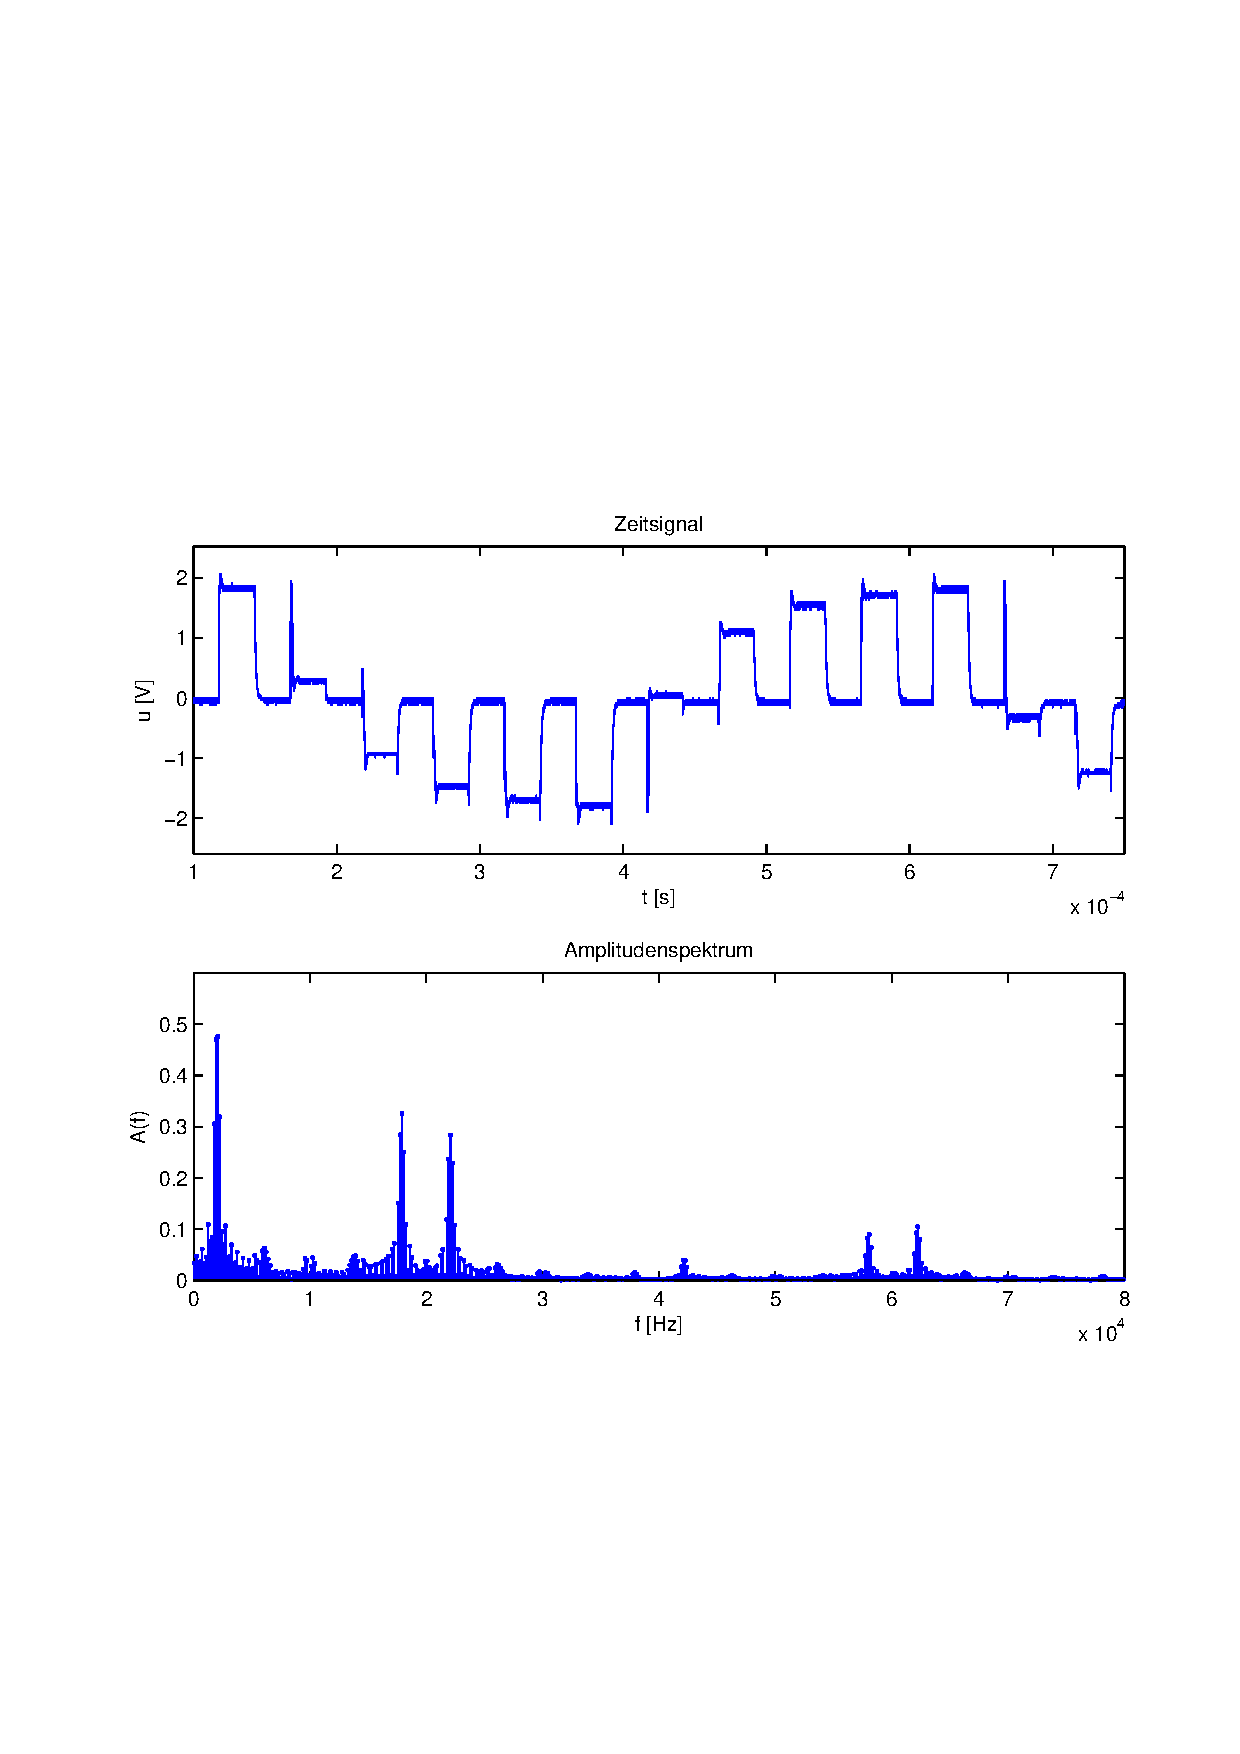
\includegraphics[scale=0.7, trim = 35mm 100mm 35mm 95mm, clip]{Bilder/flatrecFil20_05abget_zeit}
                          \caption{Flat-Top gefiltertes Rechteck moduliertes Signal}
		                  \label{fig:flatrecFil20_05zeit}
                    \end{figure}
                \end{minipage}
                
                \begin{minipage}{0.6\textwidth}
                    \begin{figure}[H]
                       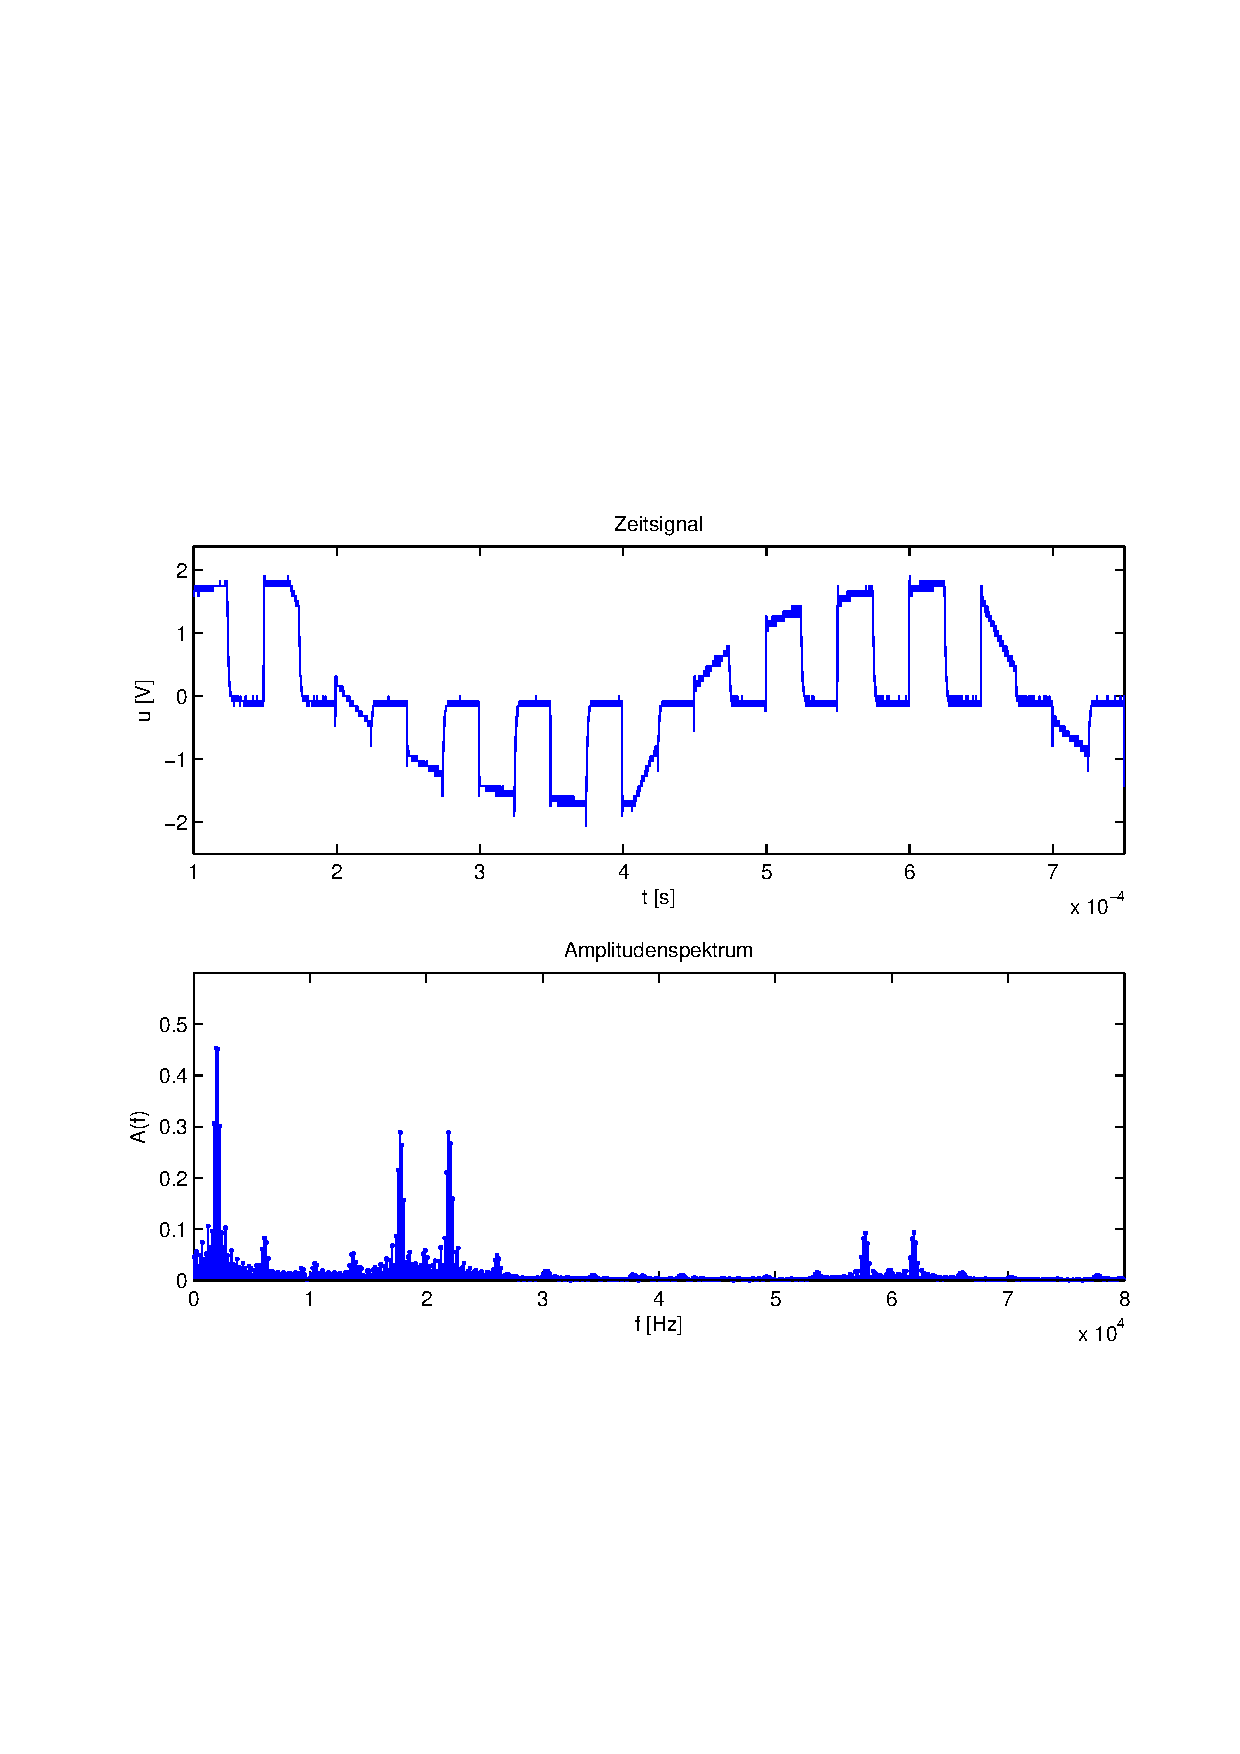
\includegraphics[scale=0.7, trim = 35mm 100mm 35mm 95mm, clip]{Bilder/shaperecFil20_05abget_zeit}
                       \caption{Shape-Top gefiltertes Rechteck moduliertes Signal}
		              \label{fig:shaperecFil20_05zeit}
                    \end{figure}
                \end{minipage}
            
            \end{tabular}
            \end{center}
            
            \begin{center}
            \begin{tabular}{ll}
            
            \hspace{-5cm}
                \begin{minipage}{0.6\textwidth}
                    \begin{figure}[H]
                        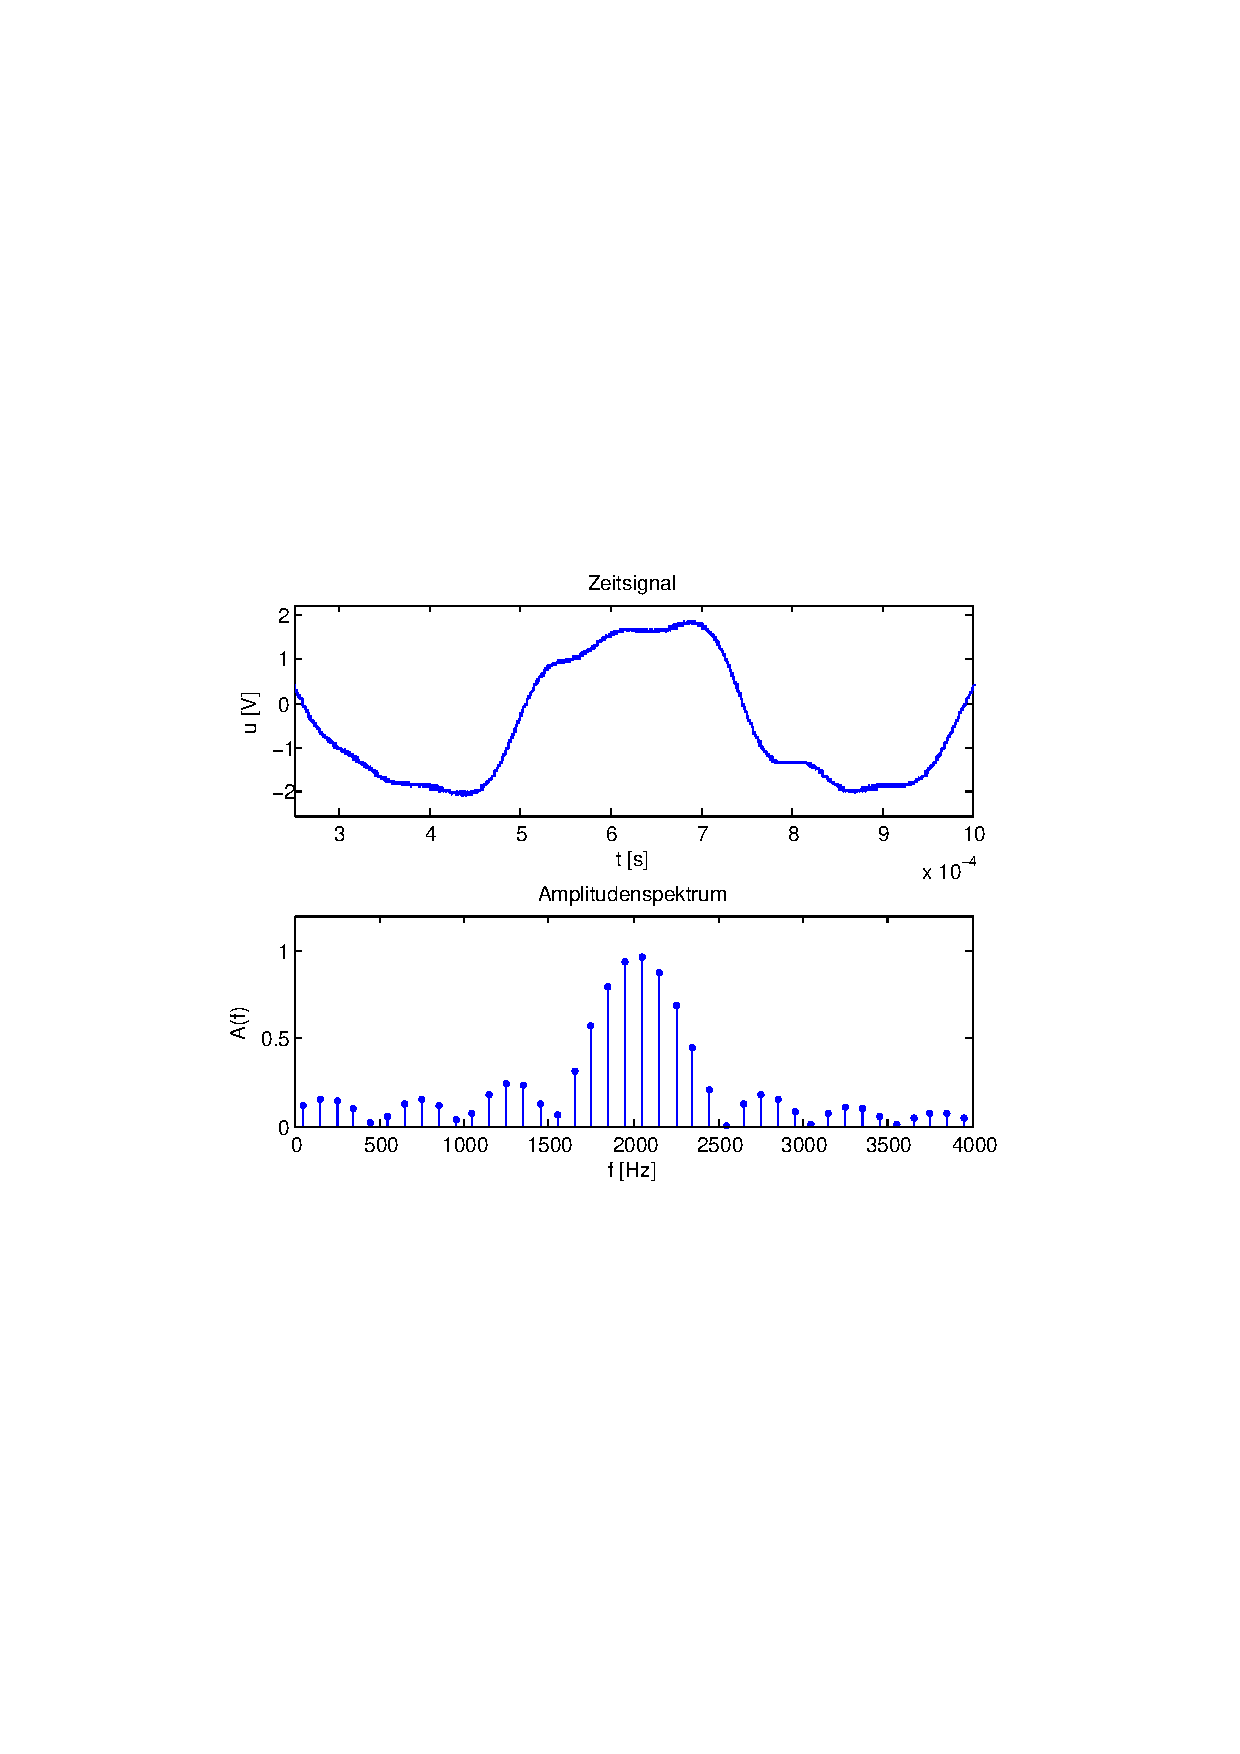
\includegraphics[scale=0.7, trim = 35mm 100mm 35mm 95mm, clip]{Bilder/flatrecFil20_05}
                          \caption{Shape-Top gefiltertes Rechteck Rekonstruktion}
		                  \label{fig:flatrecFil20_05}
                    \end{figure}
                \end{minipage}
                
                \begin{minipage}{0.6\textwidth}
                    \begin{figure}[H]
                        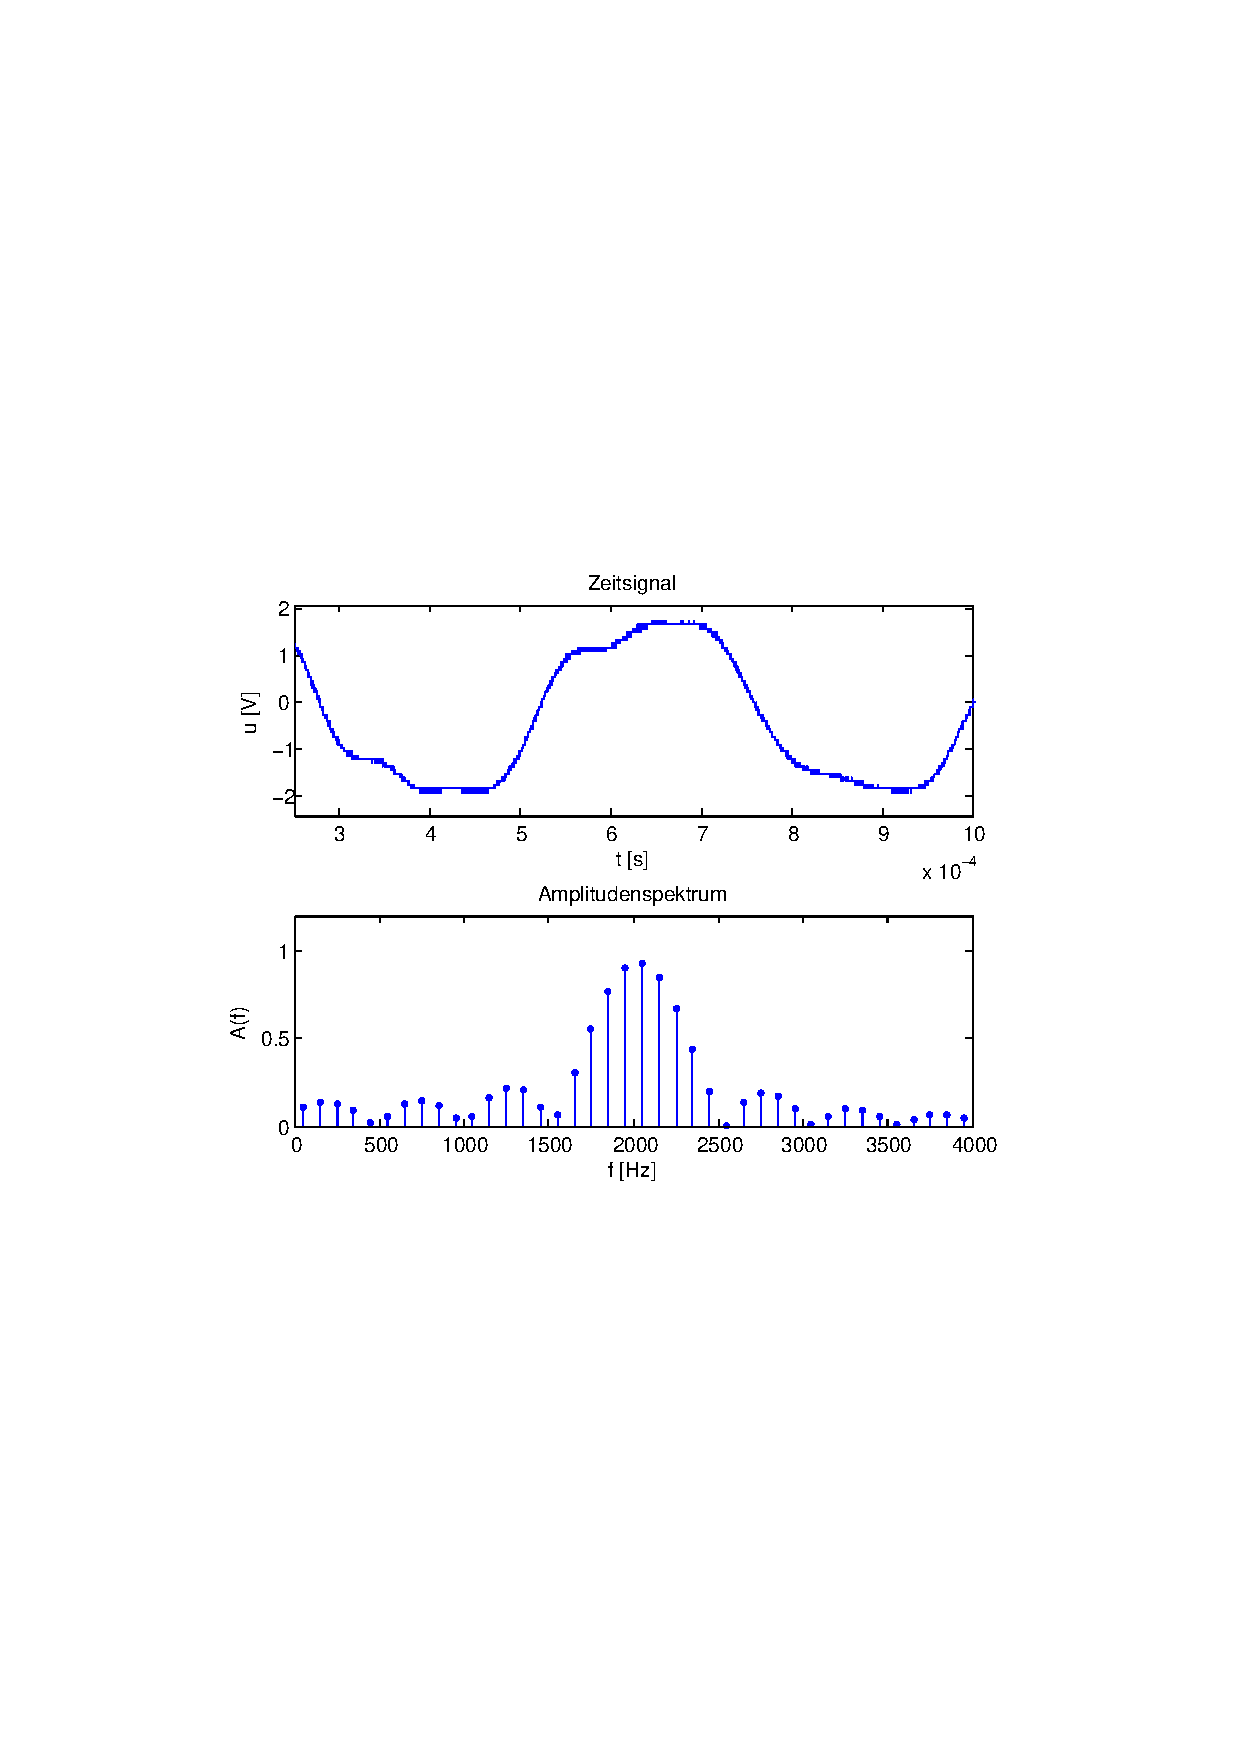
\includegraphics[scale=0.7, trim = 35mm 100mm 35mm 95mm, clip]{Bilder/shaperecFil20_05}
                       \caption{Shape-Top gefiltertes Rechteck Rekonstruktion}
		              \label{fig:shaperecFil20_05}
                    \end{figure}
                \end{minipage}
            
            \end{tabular}
            \end{center}
       
       In den Abb. \ref{fig:shaperecFil20_05zeit} und \ref{fig:flatrecFil20_05zeit} ist gut zu erkennen, dass beim
       Flat-Top Sampling, wie in der Durchführung beschrieben, ein Abtastrechteck durch das S\&H-Glied eine flache
       Oberkante hat und beim Shape-Top Sampling die Oberkante des Rechtecks der Kontur des Ausgangssignals folgt. 
       Die Rekonstruktion des Ausgangssignals ist nahezu identisch.
       Des weiteren kann man gut erkennen, dass die Filterung des Rechtecksignals vor der Abtastung eine Glättung des
       rekonstruierten Signals hervorruft und das Signal mit weniger Überschwingen rekonstruiert werden kann.
       
       Beim Flat-Top Sampling ist der Modulieraufwand auf Grund des wegfallenden S\&H-Gliedes geringer.
       
       \TODO{Was sind die Unterschiede zwischen den beiden? und was sind weitere mögliche Vorteile????}
    
      \end{quote}
      
      \subsection{Audiosignal}
      \begin{quote}
      
      \begin{center}
            \begin{tabular}{ll}
            
            \hspace{-5cm}
                \begin{minipage}{0.6\textwidth}
                    \begin{figure}[H]
                        
\includegraphics[scale=0.7, trim = 35mm 100mm 35mm 95mm, clip]{Bilder/audioflatabget_zeit}
                          \caption{Flat-Top Audiosignal moduliertes Signal}
		                  \label{fig:flataudiozeit}
                    \end{figure}
                \end{minipage}
                
                \begin{minipage}{0.6\textwidth}
                    \begin{figure}[H]
                       
\includegraphics[scale=0.7, trim = 35mm 100mm 35mm 95mm, clip]{Bilder/audioflat}
                       \caption{Flat-Top Audiosignal Rekonstruiert}
		              \label{fig:flataudio}
                    \end{figure}
                \end{minipage}
            
            \end{tabular}
            \end{center}
           
       \TODO{Warum gibt es davon kein vernünftiges abgetastetes Zeitsignal, sehen beide gleich aus was kann man
       dazu noch sagen, soll das überhaupt ins Protokoll????}
    
      \end{quote}
      
      
\end{quote}










% \begin{quote}
%     \lstinputlisting[
%         caption={Scilab-script},
%         label=lst:scilab]
%         {./Scilab/Motor.sce}
%         
% \end{quote}

%--------------------------------------------------------------------
%--------------------------------------------------------------------
% \begin{thebibliography}{999}
% 
% \bibitem{Boris}Boris Henckell: Ein Paar sachen geklaut.. ähhh inspirationen geholt
% \href{http://www.krachler.com/fileadmin/user_upload/arbeiten/Reglersynthese_Christian_Krachler.pdf}{Reglersynthese nach dem Frequenzkennlinienverfahren}, S16, S22, 08.05.2012
% 
% 
% %Name, Vorname.; evtl. Name2, Vorname2.: Titel des Dokumentes
% %oder Buches, Zeitschrift/Verlag/URL (Auflage, Erscheinungsort, -jahr), ggf. Seitenzahlen
% %\bibitem [Wiki10] {DigitaleMesskette2} \url{www.wikipedia.org}, Zugriff 22.03.2010
% \end{thebibliography}


\end{document}
